%\section{Componentes de la biblioteca \textit{MultiBody}}

%Antes de detallar la arquitectura de la biblioteca desarrollada, resulta conveniente describir los componentes de la biblioteca estándar \textit{MultiBody} que se emplearon como bloques de construcción fundamentales. Todos ellos se toman de la documentación oficial de la \textit{Modelica Standard Library} \cite{msl_multibody, otter2003}. La biblioteca \textit{MultiBody} proporciona modelos de componentes mecánicos tridimensionales (cuerpos rígidos, articulaciones y elementos de fuerza) que se interconectan de a través de un conector común, el marco de referencia.


\section{Componentes de la biblioteca \textit{Modelica\_DeviceDrivers}}

Para la comunicación entre el modelo Modelica y los sistemas externos (el visualizador y el puente de hardware) se emplea la biblioteca \textit{Modelica\_DeviceDrivers} (MDD), una biblioteca libre destinada a interconectar controladores de hardware y protocolos de comunicación con modelos de Modelica \cite{mdd}. De ella se utilizaron componentes de tres grupos funcionales: el empaquetado serializado de datos, la comunicación por UDP y la sincronización con el tiempo real. Estos bloques son los que materializan los modelos del paquete \verb|Interfaces| descritos más adelante.

\subsection*{Empaquetado de datos (\textit{SerialPackager})}

El subpaquete \verb|Packagin.SerialPackager| resuelve la serialización de datos en un formato binario transmisible para la comunicación por red. Según la documentación oficial, el objetivo del \textit{SerialPackager} es permitir agregar y recuperar datos de un paquete de manera independiente del dispositivo \cite{mdd}. Los bloques se encadenan a través de conectores (\verb|pkgIn| y \verb|pkgOut|) que representan un buffer de paquete a compartir, el cual va siendo construido o desarmado a medida que se recorre la cadena.


\subsubsection{Packager}
Es el bloque de cabecera de la cadena: inicializa el búfer del paquete sobre el que los bloques posteriores escriben o del que leen.

\subsubsection{AddFloat}

Toma un vector de valores \verb|Real| y los convierte en un número de punto flotante de $32$ bits para luego añadirlos al paquete. El parámetro \verb|nu| indica el número de entradas. Se emplea del lado emisor para serializar las coordenadas y/o señales.



\subsubsection{GetFloat} 
Realiza la operación inversa a \verb|AddFloat|, extrae un vector de números de punto flotante del paquete recibido y los convierte a doble precisión antes de asignarlo a un arreglo \verb|Real| de Modelica \cite{mdd}. Se emplea del lado receptor para obtener las señales entrantes

\subsection*{Comunicación por UDP}

El subpaquete \verb|Communication| provee los bloques de entrada y salida de red que transportan el paquete serializado a través del protocolo UDP.



\subsubsection{UDPSend}
Bloque que permite el envío de datagramas UDP hacia la red. Recibe el paquete ensamblado a través de su conector \verb|pkgIn| y lo emite como un datagrama hacia el puerto \verb|port_send| con un período definido por \verb|sampleTime|. Es el bloque final de la cadena de transmisión.



\subsubsection{UDPReceive}
Bloque que permite la recepción de datagramas UDP. Escucha en el puerto definido por \verb|port_recv|, mediante un hilo de recepción en el segundo plano y expone los bytes serializados recibidos a través de su conector \verb|pkgOut| para que luego los bloques \verb|GetFloat| los desempaqueten. Es el bloque inicial de la cadena de recepción.

\subsection*{Sincronización con el tiempo real}



\subsubsection{RealtimeSynchronize}
Este bloque se encarga de la sincronización del tiempo de la simulación con el reloj de tiempo real del sistema operativo. Su funcionamiento consiste en comparar, mediante una función externa en C, el tiempo de simulación con el reloj del sistema, deteniendo la ejecución del hilo hasta que el primero alcanza al segundo. Es indispensable para que una simulación que podría ejecutarse más rápid que el tiempo real se ajuste al ritmo del mundo físico, condición necesaria tanto para una visualización fiel, como para cerrar el feedback del conductor. La documentación advierte de que se trata de una sincronización blanda (\textit{soft real-time}) no apta para aplicaciones de tiempo real estricto ni de seguridad crítica \cite{mdd}, pero para un simulador de conducción interactivo, esta aproximación me pareció suficiente. El bloque admite ademas un modo muestreado (\textit{sampled}) que ofrece un comportamiento más determinista y menos sensible al solver.

En conjunto, estos bloques se utilizan en dos sentidos:  en la transmisión, \verb|Packager| $\rightarrow$ \verb|AddFloat| (uno por señal) $\rightarrow$ \verb|UDPSend|, y en la recepción, \verb|UDPReceive| $\rightarrow$ \verb|GetFloat| (uno por señal), todo ello sincronizado por \verb|RealtimeSynchronize|.

\section{Biblioteca de dinámica vehicular}

En esta sección se explicará el desarrollo y arquitectura de la biblioteca de dinámica vehicular implementada en Modelica. Para garantizar la modularidad y facilitar el mantenimiento y evolución del código, la bilbioteca se organizó en tres paquetes principales:


\begin{itemize}
    \item \verb|Roads|: Contiene la lógica referida al entorno de la simulación, incluyendo características topológicas de la pista/circuito y la geometría de la superficie de contacto.
    \item \verb|Interfaces|: Define los conectores estandarizados y los protocolos de comunicación, permitiendo la comunicación fluida entre los diferentes subsistemas y la compatibilidad con componentes externos.
    \item \verb|Cars|: Agrupa los modelos físico-matemáticos correspondientes a la topología del vehículo, en este paquete se incluye el detalle de la cinemática del chasis, los sistemas de suspensión y demás elementos mecánicos estructurales, entre otras cosas.
\end{itemize}

\subsection{Interfaces}

El paquete \verb|Interfaces| actúa como capa de compatibilidad entre el dominio mecánico de la bibliotecta \textit{MultiBody} y los dominios de las señales de entrada del piloto y de la comunicación de red. Su función es tanto extraer información de estado del modelo físico y ponerla a disposición de otros subsistemas, ya sea como señales continuas internas o como datagramas transmitidos en tiempo real hacia un cliente externo mediante UDP, como permitir la recepción de señales pertenecientes a los inputs del vehículo, también mediantes datagramas UDP. Este paquete contiene dos familias de modelos: los que transmiten únicamente la posición (\verb|FrameToReal| y \verb|FrameToUDP|) y los que además transmiten la orientación del marco de referencia (\verb|FrameToRealOrientation| y \verb|FrameToUDPOrientation|), necesarios para reproducir en el visualizador la dirección del vehículo y el giro de las ruedas. A estos transmisores se suma un modelo de recepción, \verb|UDPInput|, que implementa el canal inverso: la lectura de los comandos del conductor enviados por la interfaz de hardware.\\

\subsubsection{FrameToReal}

El modelo \verb|FrameToReal| cumple con la función de sensor de posición sobre un conector \verb|Frame_a| de la biblioteca \textit{MultiBody}. Este marco transporta, entre sus componentes, el vector de posición en el sistema de referencia global $\mathbf{r}_0 \in \mathbb{R}^3$, así como las fuerzas y torques aplicados sobre este. Dado que el modelo tiene carácter observacional, las ecuaciones extraen las componentes cartesianas del vector de posición y las asignan a tres salidas de señal continua, de tipo \verb|Real|, sin aplicar ni fuerza ni torque sobre el frame, para garantizar que no se introducen variaciones inesperadas en el sistema::

\begin{align}
    x_{\text{out}} &= r_{0,1} \\
    y_{\text{out}} &= r_{0,2} \\
    z_{\text{out}} &= r_{0,3} \\
    \mathbf{f} &= \mathbf{0} \\
    \boldsymbol{\tau} &= \mathbf{0}
\end{align}

Las tres salidas son de tipo \verb|RealOutput| (pertenecientes a \verb|Modelica.Blocks.Interfaces|), lo que las hace directamente compatibles con cualquier bloque de procesamiento de señales del ecosistema Modelica.\\

\subsubsection{FrameToUDP}

El modelo \verb|FrameToUDP| construye sobre la funcionalidad de \verb|FrameToReal|, agregando una cadena de serialización y transmisión de datos por red basada en la biblioteca \verb|Modelica_DeviceDrivers|. Su objetivo es enviar la posición del vehículo a un cliente externo, en este caso, a el motor gráfico Unity, mediante el protocolo UDP, permitiendo la visualización en tiempo real del estado del sistema/vehículo. \\

Por dentro, el modelo encadena los siguientes componentes: \verb|FrameToReal| que extrae las tres coordenadas del marco de referencia como variables \verb|Real|, un bloque \verb|Packager| que inicializa el buffer del datagrama, tres instancias de \verb|AddFloat| que agregan cada coordenada como un número de punto flotante de 32 bits en formato IEEE 754 little-endian \cite{mdd}, finalmente, \verb|UDPSend| transmite el paquete resultante al puerto 12345 (configurable) con un período de muestreo de 
0{,}01 s, es decir a una frecuencia de 100Hz, esta frecuencia puede ser aumentada para mejorar la fidelidad de la simulación a cambio de necesitar más poder de procesamiento.

Como fue explicado en la sección de \textit{DeviceDrivers}, el paquete también incluye un componente adicional \verb|RealtimeSynchronize|, que sincroniza el reloj de la simulación con el reloj del sistema operativo. Esta sincronización es indispensable para que la frecuencia de los datagramas corresponda efectivamente a 100 paquetes (o lo configurado) por segundo en tiempo real, garantizando así, la coherencia entre el modelo de Modelica y el visualizador utilizado.\\

\subsubsection{FrameToRealOrientation}

Transmitir solamente la posición resulta insuficiente cuando se quiere representar la actitud del vehículo o el ángulo de dirección de las ruedas en el visualizador. El conector \verb|Frame_a| transporta, además del vector de posición $\mathbf{r}_0$ ya utilizado, un objeto de orientación $R$ que contiene la matriz de transformación $T \in \mathbb{R}^{3\times3}$ entre el sistema de referencia global y el sistema local del cuerpo. El modelo \verb|FrameToRealOrientation| extiende a \verb|FrameToReal| exponiendo, junto a las tres coordenadas de posición, dicha orientación en forma de cuaternión unitario.\\

Se optó por representar la orientación mediante un cuaternión y no por la matriz de rotación completa (nueve componentes) ni por ángulos de Euler, ya que el cuaternión requiere solo cuatro componentes, evita singularidades y es el formato nativo de rotación en Unity. La conversión se realiza con la función \verb|Frames.to_Q| de la biblioteca \textit{MultiBody}, que aplica la convención $\mathbf{Q} = [\sin(\theta/2)\,\hat{\mathbf{e}};\ \cos(\theta/2)]$, con la parte escalar en la última componente:

\begin{align}
    x_{\text{out}} &= r_{0,1} \\
    y_{\text{out}} &= r_{0,2} \\
    z_{\text{out}} &= r_{0,3} \\
    \mathbf{q}_{\text{out}} &= \text{to\_Q}(R) \\
    \mathbf{f} &= \mathbf{0} \\
    \boldsymbol{\tau} &= \mathbf{0}
\end{align}



Cabe destacar que $\text{to\_Q}(R)$, devuelve la rotación del cuerpo respecto del mundo expresada como cuaternión activo. El script que actúa como cliente receptor del lado de Unity convierte esta rotación al sistema de Unity aplicando la misma inversión de eje que a la posición, lo que equivale a negar las componentes $x$ e $y$ de la parte vectorial y conservar $z$ y $w$. Es importante destacar que negar la componente $z$ en su lugar produce la rotación inversa, lo que se ve reflejado como una representación errónea del movimiento del eje de giro de la rueda, cosa que fue una fuente de complicaciones durante el desarrollo.\\

\subsubsection{FrameToUDPOrientation}

El modelo \verb|FrameToUDPOrientation| es el equivalente a \verb|FrameToUDP| pero para la transmisión de la localización completa. Reemplaza el objeto \verb|FrameToReal| por \verb|FrameToRealOrientation| y amplía la cadena de serialización para incluír siete números en total de punto flotante en $32$ bits:
 las tres coordenadas de posición y las cuatro componentes del cuaternión. El puerto de destino (\verb|port_send|) y el período de muestreo (\verb|sampleTime|) se declaran como parámetros, lo que permite, además de intercambiar fidelidad por performace, instanciar varias transmisores al mismo tiempo, por ejemplo, incluyendo uno para el chasis y otros cuatro, uno para cada rueda, todos dirigidos a puertos distintos.\\

Cada valor se serializa mediante un bloque \verb|AddFloat| independiente encadenado en secuencia, en lugar de un único bloque configurado para siete valores. Esta decisión se tomó debido a una limitación observada en el compilador OpenModelica~1.25.5, en el que la modificación del parámetro de tamaño del bloque \verb|AddFloat| provoca un error interno de instanciación, el encadenamiento de bloques con el tamaño por defecto evita dicho comportamiento.\\

Dado que en la topología del vehículo los frames de las ruedas se ubican sobre la salida de la junta de rotación, la orientación transmitida incluye tanto el ángulo de dirección como el giro propio de la rueda, permitiendo que sea representada de forma correcta por el entorno gráfico. El ejemplo \verb|CarExampleUDP| demuestra este sistema, instanciando el vehículo y el entorno y aplicando una señal de dirección para probar el giro de la dirección y conecta cinco transmisores \verb|FrameToUDPOrientation| (chasis y cuatro ruedas) a puertos consecutivos del 12345 al 12349.\\

\subsubsection{UDPInput}

El modelo \verb|UDPInput| implementa el canal de comunicación de recepción del sistema, permitiendo obtener los comandos del conductor. Constituye la contraparte en Modelica de la aplicación de adquisición de datos desde el hardware descrita en la sección \textit{Interfaz para el hardware}, y cierra el lazo \textit{Man-in-the-Loop} al incluir en el modelo las acciones ejercidas por el piloto capturadas desde los periféricos.\\

Su estructura interna es simétrica a la de \verb|FrameToUDP|, pero orientada a la lectura: un bloque \verb|UDPReceive| escucha en el puerto configurable \verb|udpPort| (por defecto, 12347) y entrega el datagrama UDP recibido, para que luego, cuatro bloques \verb|GetFloat| desempaqueten la información y la codifiquen en cuatro números de punto flotante de $32$ bits, convirtiéndolos luego a variables \verb|Real| de doble precisión. Estas son expuestas como cuatro salidas \verb|RealOutput|: \verb|steer|, \verb|throttle|, \verb|brake| y \verb|clutch|, que se conectan respectivamente a las entradas \verb|steerInput|, \verb|throttleInput| y \verb|brakeInput| del modelo del vehículo (la señal de embrague queda disponible para usos futuros si se considerase necesaria). El formato de 16 bytes y el puerto 12347 coinciden exactamente con los que emite la aplicación \verb|FFBReceiver|, garantizando la conexión fluída entre ambos extremos. Al igual que los transmisores, incorpora un bloque \verb|RealtimeSynchronize| para sincronizar la recepción en tiempo real.\\

\subsection{Roads}

El paquete \verb|Roads| encapsula el entorno y el mundo de la simulación sobre el que opera el vehículo. Sus responsabilidades principales incluyen: por un lado, definir la geometría de la superficie de contacto que va a actuar como pista, y por otro, calcular y aplicar las fuerzas mecánicas generadas por la interacción entre cada neumático y dicha superficie. Este paquete se organiza en tres niveles: el modelo integrador \verb|Road|, el subpaquete \verb|Floor| que incluye los modelos de contacto entre la rueda y la superficie, y el subpaquete \verb|Terrains| que gestiona la definición y visualización del terreno.\\


\subsubsection{Road}

El modelo \verb|Road| es el componente de más alto nivel del paquete y actúa como punto de ensemble para el entorno completo. Instancia, primero, un objeto \verb|World| de la biblioteca \textit{MultiBody}, necesario para definir un sistema de referencia global y el vector de gravedad, junto con un \verb|TerrainMap| y un \verb|Floor4Corners|. Tanto \verb|World| como \verb|TerrrainMap| se declaran como objetos \texttt{inner}, lo que permite que cualquier submodelo del sistema los referencia mediante la palabra reservada \texttt{outer} sin necesidad de pasarlos como argumentos. \\

Hacia el resto del modelo, \verb|Road| expone cuatro conectores de tipo \verb|Frame_a|, uno perteneciente a cada esquina del vehículo: delantera izquierda (\verb|FL|), delantera derecha (\verb|FR|), trasera izquierda (\verb|RL|) y trasera derecha (\verb|RR|). Estos frames se conectan directamente con los de los centros de rueda del modelo del vehículo, constituyendo la conexión mecánica entre el entorno/mundo de simulación y el chasis.\\


\subsubsection{Floors}

El subpaquete \verb|Floors| implementa el modelo de contacto entre la rueda y el suelo mediante una jerarquía de tres clases. Arriba, \verb|Floor4Corners| agrega cuatro instancias del modelo \verb|Floor|, una por rueda, y les pasa a cada uno un conjunto de parámetros físicos compartidos: la rigidez del suelo \verb|ground_c| ($c = 10^5$ N/m), el coeficiente de amortiguamiento normal \verb|ground_d| ($d = 5000$ N$\cdot$s/m), el coeficiente de fricción longitudinal \verb|ground_mu| ($\mu_\text{long} = 10000$ N$\cdot$s/m) y el coeficiente de fricción lateral \verb|mu_lat| ($\mu_\text{lat} = 100000$ N$\cdot$s/m). El radio de la rueda \verb|R_wheel| se propaga hacia abajo mediante cláusulas \texttt{inner}/\texttt{outer} desde el nivel de simulación. \\

El modelo \verb|Floor| es un modelo compuesto que instancia dos subcomponentes, \verb|GroundSpring| y \verb|GroundFriction|, compartiando el mismo conector de contacto \verb|wheelContact|, de tipo \verb|Frame_b|. \\

\subsubsection{GroundSpring}
Este componente aplica la fuerza normal vertical, utilizando un modelo de resorte-amortiguador lineal. La fuerza aplicada es nula mientras el centro de la rueda (más su radio) se encuentre por encima de la superficie del terreno, y crece de forma proporcional a la profundidad de penetración del neumático. La ley de fuerza utilizada es \cite{gillespie1992}:

\begin{equation}
    F_y = \max\!\left(0,\; c \cdot \bigl[\,h(x, z) + R_\text{wheel} - y\,\bigr] - d \cdot \dot{y}\right)
\end{equation}

donde $h(x, z)$ es la altura del terreno en la posición horizontal del contacto, obtenida a través del objeto \texttt{outer terrain}, $y$ es la coordenada vertical del centro de la rueda en el sistema de referencia global, $\dot{y}$ su velocidad vertical y $R_{wheel}$ es el radio de la rueda. El operador $\max(0, \cdot)$ garantiza que el suelo solo empuja y nunca tracciona. \\

\subsubsection{GroundFriction}

Este componente calcula las fuerzas de fricción longitudinal y lateral en el punto de contacto, controlando el agarre que tienen las ruedas con el suelo. La dirección de avance (\textit{heading}) y la dirección del eje de la rueda (\textit{axle}) se determinan directamente a partir de la matriz de rotación del marco de contacto. A partir de ellas se calcula primero una demanda de fricción $\mathbf{F}_\text{dem}$, con una componente longitudinal de tipo \textit{slip}, proporcional a la diferencia entre la velocidad de traslación de la rueda en la dirección de avance y la velocidad  impuesta por su rotación, y una componente lateral viscosa :

\begin{equation}
    \mathbf{F}_\text{dem} = f_\text{ramp} \Bigl[ -\mu_\text{long}\,\bigl(v_\text{long} - \omega_z\, R_\text{wheel}\bigr)\, \hat{\mathbf{e}}_\text{heading} \;-\; \mu_\text{lat}\, v_\text{lat}\, \hat{\mathbf{e}}_\text{axle} \Bigr]
\end{equation}

donde $f_\text{ramp}$ (\verb|frictionScale|) es un factor lineal que hace crecer la fuerza desde cero hasta su valor máximo en función de la profundidad de penetración, evitando discontinuidades en el instante de contacto.\\

Sobre esta demanda se impone un límite de \textit{círculo de fricción} (\textit{friction circle}): la fuerza de contacto combinada no puede superar $\mu_\text{peak} \cdot N$, donde $N$ es la carga normal estimada en el parche y $\mu_\text{peak}$ el coeficiente de fricción pico (por defecto $1{,}0$). La carga normal se obtiene recomputando la misma fórmula resorte-amortiguador empleada en \verb|GroundSpring|:

\begin{equation}
    N = \max\!\left(0,\; c \cdot \bigl[\,h(x, z) + R_\text{wheel} - y\,\bigr] - d \cdot \dot{y}\right)
\end{equation}

y la fuerza final se obtiene saturando la demanda a dicho límite, conservando su dirección:

\begin{equation}
    \mathbf{F}_\text{friction} =
    \begin{cases}
        \mathbf{F}_\text{dem} & \text{si } \|\mathbf{F}_\text{dem}\| \le \mu_\text{peak}\, N \\[6pt]
        \mu_\text{peak}\, N \cdot \dfrac{\mathbf{F}_\text{dem}}{\|\mathbf{F}_\text{dem}\|} & \text{si } \|\mathbf{F}_\text{dem}\| > \mu_\text{peak}\, N
    \end{cases}
\end{equation}

Este mecanismo hace que las direcciones longitudinal y lateral compartan una cantidad limitada de agarre: una aceleración o una frenada intensa reducen la fuerza lateral disponible para el giro, y viceversa, tal como ocurre en un neumático real \cite{milliken1995,gillespie1992}. Además, limita el agarre lateral máximo, evitando fuerzas de contacto irreales que podrían generar vuelcos, y permite que el vehículo pueda subvirar o sobrevirar al quedarse sin agarre. Por debajo del límite, el comportamiento coincide con el modelo viscoso, por encima, el neumático desliza y la fuerza se satura en lugar de crecer sin cota. Para que la estimación de $N$ sea coherente, los coeficientes $c$ y $d$ deben coincidir con los de \verb|GroundSpring|, lo que \verb|Floor| y \verb|Floor4Corners| garantizan al distribuir los mismos valores a ambos submodelos.\\

% Finalmente, el torque resultante de aplicar la fricción a nivel del parche de contacto (utilizando el radio del neumático definido como $R_\text{wheel}$) se computa mediante el producto vectorial: 

% \begin{equation}
%     \boldsymbol{\tau} = \{0,\, -R_\text{wheel},\, 0\} \times \mathbf{F}_\text{friction}
% \end{equation}

% Este torque es el responsable de transmitir la fuerza de tracción como par rotacional sobre la articulación de la rueda, cerrando el circuito entre la dinámica traslacional del chasis y la dinámica rotacional del neumático.\\



% \subsubsection*{Resistencia a la rodadura} 
A la fuerza de fricción se le suma la resistencia a la rodadura que se genera cuando la carcasa se deforma al entrar en contacto con la superficie y no devuelve toda la energía al salir, lo que resulta como una fuerza retardadora proporcional a la carga normal \cite{gillespie1992}. Su magnitud se modela mediante un coeficiente adimensional $C_\text{rr}$, con valores típicos entre $0{,}010$ y $0{,}015$ para un neumático de automóvil sobre asfalto:

\begin{equation}
    \mathbf{F}_\text{rr} = -C_\text{rr}\, N \, \tanh\!\left(\frac{v_\text{long}}{v_\text{rr}}\right) \hat{\mathbf{e}}_\text{heading}
\end{equation}

% Dos decisiones de modelado merecen justificación. La primera es que esta fuerza se añade \textit{después} de la saturación del círculo de fricción y no dentro de la demanda $\mathbf{F}_\text{dem}$. La resistencia a la rodadura no es una fuerza de Coulomb y por tanto no compite por el mismo presupuesto de agarre: incluirla en la demanda implicaría que un neumático deslizando en el límite de adherencia perdiera su pérdida por histéresis, lo cual es físicamente incorrecto.\\

Una decisión que merece ser justificada es la regularización mediante $\tanh$. La ley física original es $-C_\text{rr} N \operatorname{sign}(v_\text{long})$ \cite{gillespie1992}, que presenta una discontinuidad de salto exactamente en $v_\text{long} = 0$, es decir, cuando el vehículo está detenido. Una discontinuidad en este punto obliga al integrador a reducir el paso indefinidamente o a oscilar entre ambas ramas. El parámetro $v_\text{rr} = 0{,}3$ m/s define el ancho de la transición suave: a menor valor, la simulación es más fiel a la ley ideal, pero endurece el sistema numéricamente. Se emplea el mismo método que en \verb|DiscBrake| para el mismo problema. Dado que $N$ ya es nula fuera del contacto por el operador $\max(0, \cdot)$, la fuerza de rodadura se anula automáticamente cuando la rueda pierde el suelo.\\

La fuerza total en el parche es entonces la suma de ambas fuerzas, $\mathbf{F}_\text{contact} = \mathbf{F}_\text{friction} + \mathbf{F}_\text{rr}$ Finalmente, el torque de rodadura resultante de aplicar dicha fuerza a nivel del parche de contacto (a una distancia $R_\text{wheel}$ por debajo del centro de la rueda) se computa mediante el producto vectorial:

\begin{equation}
    \boldsymbol{\tau} = \{0,\, -R_\text{wheel},\, 0\} \times \mathbf{F}_\text{contact}
\end{equation}


Este torque es el responsable de transmitir la fuerza de tracción como par rotacional sobre la articulación de la rueda, cerrando el ciclo entre la dinámica traslacional del chasis y la dinámica rotacional del neumático. Al incluir la resistencia a la rodadura, se obtiene además el par retardador que frena una rueda en rodadura libre, de modo que el vehículo en punto muerto desacelera hasta frenar en lugar de seguir avanzando indefinidamente.\\

\subsubsection{Terrains}

El subpaquete \verb|Terrains| gestiona la definición de la geometría del terreno que va a actuar como pista y su representación visual. El bloque \verb|TerrainMap| expone la función \verb|getZ(x, y)| que devuelve la altura de la superficie en cualquier coordenada horizontal del mundo. Esta función es llamada en cada paso de la integración, tanto por \verb|GroundSpring| como por \verb|GroundFriction| a través del objeto \texttt{outer terrain}. Las implementaciones actuales pueden devolver, o un plano horizontal constante a $y = 1$ m, u otro definido por una función $y = sen(x)$. Sin embargo, es sencillo agregar nuevas expresiones analíticas o tablas de datos para representar diferentes tipos de terrenos.\\

La función \verb|terrainSurface|, perteneciente al subpaquete \verb|Components|, implementa la interfaz 
\verb|partialSurfaceCharacteristic| de \textit{MultiBody} y genera la malla de vértices que \verb|TerrainVisualizer| renderiza en la animación 3D incluída dentro del propio visualizador de OpenModelica. Es necesario mantener su comportamiento sincronizado con \verb|TerrainMap.getZ| para que la representación visual sea consistente con la geometría utilizada en el cálculo de fuerzas. Por otro lado, \verb|TerrainVisualizer| extiende \verb|PartialVisualizer| y representa el suelo como un plano sólido en la animación del entorno de OpenModelica, conectándose al marco de referencia del \verb|World|. Sin embargo, por limitaciones del compilador OpenModelica a la hora de renderizar curvas, esta función no se utiliza y se deja como placeholder. Este visualizador se utiliza solo como herramienta de debugging, ya que la visualización del sistema se realiza en un motor externo, en este caso en Unity.\\


\subsubsection{Aerodynamics}

El subpaquete \verb|Aerodynamics| incorpora la interacción del vehículo con el aire del entorno, este paquete es una simplificación de un modelo aerodinámico realista, ya que implementar algo de ese calibre requeriría conocimiento, poder de cómputo y tiempo fuera del alcance de esta tesina. Sin esta resistencia, el vehículo aceleraría de forma indefinida bajo un comando de acelerador constante, la componente aerodinámica es la dominante de las resistencia a altas velocidades, y es la que limita la velocidad máxima del vehículo.\\

\subsubsection{AeroDrag} Este componente aplica una fuerza de arrastre cuadrática sobre el marco de referencia al que se conecta. La ley de fuerza es la expresión clásica del arrastre aerodinámico \cite{gillespie1992}:

\begin{equation}
    \mathbf{F}_\text{drag} = -\tfrac{1}{2}\, \rho\, C_d\, A\, \lVert \mathbf{v} \rVert\, \mathbf{v}
\end{equation}

donde $\rho = 1{,}2$ kg/m$^3$ es la densidad del aire, $C_d$ el coeficiente de arrastre, $A$ el área frontal de referencia y $\mathbf{v}$ la velocidad absoluta del frame resuelta en el sistema global. Al formularse de forma vectorial y no únicamente sobre la dirección de avance, la fuerza se opone al movimiento en los tres ejes, amortiguando también los desplazamientos laterales y verticales. Internamente el modelo instancia un sensor \verb|AbsoluteVelocity| y un elemento \verb|WorldForce|, ambos conectados al mismo \verb|Frame_a|.\\

La velocidad de equilibrio que introduce esta fuerza se obtiene igualando arrastre aerodinámico y tracción, y define la velocidad máxima del vehículo:

\begin{equation}
    v_\text{max} = \sqrt{\frac{2\,F_\text{tracción}}{\rho\, C_d\, A}}
\end{equation}

\begin{equation}
    F_\text{tracción} = \frac{\tau}{R_\text{wheel}}, \qquad \tau = \verb|torqueValue| \cdot \verb|pedalInput|
\end{equation}




% \paragraph{Regularización numérica.} El módulo de la velocidad se calcula como $\lVert \mathbf{v} \rVert = \sqrt{\mathbf{v}\cdot\mathbf{v} + v_\text{reg}^2}$ en lugar de $\sqrt{\mathbf{v}\cdot\mathbf{v}}$. El motivo es que, aunque el producto $\lVert \mathbf{v} \rVert \mathbf{v}$ es de clase $C^1$ en el origen, su jacobiano contiene el término $\mathbf{v}\otimes\mathbf{v} / \lVert \mathbf{v} \rVert$, indeterminado en $\mathbf{v} = \mathbf{0}$; y precisamente el vehículo parte del reposo, de modo que el integrador encuentra ese punto en el primer paso. El valor por defecto $v_\text{reg} = 0{,}1$ m/s mantiene el jacobiano acotado a cambio de una fuerza residual a baja velocidad muy inferior a la resistencia a la rodadura.\\

% \subsubsection*{Parametrización por vehículo.} 
Cada modelo de vehículo instancia su propio \verb|AeroDrag| conectado al frame del chasis, con los valores correspondientes al vehículo en el que se basa: $C_d = 0{,}70$ y $A = 1{,}10$ m$^2$ para \verb|Car|, un monoplaza de ruedas descubiertas, cuya resistencia está definida por los neumáticos expuestos, $C_d = 0{,}36$ y $A = 1{,}90$ m$^2$ para \verb|CivicEKCar|, y $C_d = 0{,}32$ y $A = 1{,}95$ m$^2$ para \verb|E36Car|.\\

Queda fuera del alcance de esta tesina la carga aerodinámica vertical (\textit{downforce}), el desplazamiento del centro de presiones respecto del centro del chasis (razón por la que el arrastre no genera momento de cabeceo), la dependencia de $C_d$ con el ángulo de guiñada, y la presencia de viento, el aire se supone en reposo respecto del sistema global.\\

Quedan fuera del alcance del modelo actual la sustentación y la carga aerodinámica vertical (\textit{downforce}), el desplazamiento del centro de presiones respecto del origen del marco del chasis (razón por la que el arrastre no genera momento de cabeceo), la dependencia de $C_d$ con el ángulo de guiñada, y la presencia de viento: el aire se supone en reposo respecto del sistema global.\\

\subsection{Cars}

El paquete \verb|Cars| contiene los modelos del vehículo y todos los subsistemas que lo componen. Está organizado de la siguiente forma: en el nivel superior, se encuentran los modelos de vehículo completos, mientras que el subpaquete \verb|Parts| contiene los partes necesarias para construir dichos modelos: chasis, suspensiones, neumáticos, diferencial y frenos. Todos estos subcomponentes siguen un patrón de diseño orientado a objetos, con clases parciales que definen una interfaz y parámetros comunes, sobre las cuales se implementan las clases concretas.\\

\subsubsection*{Modelos de vehículo completos}

Los vehículos de alto nivel utilizan y conectan todos los subcomponentes del paquete \verb|Parts|, exponiendo hacia el exterior solamente los conectores necesarios para la interacción con el piloto y el entorno de simulación.\\

La interfaz exterior es la misma en todos los modelos: cuatro conectores  \verb|Frame_a|, \verb|frame_FL|, \verb|frame_FR|, \verb|frame_RL|, \verb|frame_RR|, para el contacto con el \verb|Road|, un conector \verb|chassis_pos|, utilizado para obtener la ubicación del chasis y tres entradas normalizadas que representan los comandos del conductor: \verb|steerInput| (comando de dirección en $[-1, 1]$, donde $-1$ corresponde al tope izquierdo y $+1$ al derecho), \verb|throttleInput| (comando de acelerador en $[0, 1]$) y \verb|brakeInput| (comando de frenado en $[0, 1]$). Estos comandos normalizados no actúan directamente sobre la mecánica, ya que son traducidos a magnitudes físicas por los subsistemas de dirección (\verb|Steering|) y transmisión (\verb|Transmission|) descritos más adelante, sin embargo, actualmente estos sistemas tienen implementaciones \verb|Mock| para evitar complejizar más el modelo. La posición inicial del chasis se establece a través de una articulación \verb|FreeMotion| conectada al \verb|World|, con condición inicial de altura $y_0 > 0$ para que el vehículo arranque suspendido sobre el terreno y caiga libremente hasta el equilibrio estático.\\


La biblioteca incluye tres modelos de vehículo parametrizados:

\begin{itemize}
    \item \verb|Car|: vehículo genérico de tracción trasera. Chasis rectangular de 400 kg (3{,}0 m $\times$ 1{,}8 m $\times$ 0{,}5 m), suspensión \verb|DoubleWishbone| en las cuatro puntas (par delantero con dirección), \verb|Tire| pasivo delante y \verb|DrivingTire| detrás, diferencial \verb|SolidAxle|. Basado en un Formula Ford 1600.
    \item \verb|CivicEKCar|: Basado en un Honda Civic EK hatchback de tracción delantera. 990 kg de masa suspendida, batalla 2620 mm, \verb|DoubleWishbone| en todas las esquinas (rigidez 16 kN/m delantera / 14 kN/m trasera, amortiguamiento 1800 N$\cdot$s/m), neumático 185/65R14 ($R = 0{,}30$ m).
    \item \verb|E36Car|:  Basado en un BMW E36 de tracción trasera. 1000 kg de masa suspendida, batalla 2700 mm, \verb|McPherson| delante (20 kN/m, 2200 N$\cdot$s/m) y \verb|MultiLink| detrás (16 kN/m, 2200 N$\cdot$s/m), neumático 195/65R15 ($R = 0{,}31$ m).
\end{itemize}

\subsubsection*{Parts.Chassis}

El subpaquete \verb|Chassis| define la estructura del chasis del vehículo. La clase parcial \verb|BaseChassis| establece la interfaz mínima: un parámetro para fijar la masa $m$ y un único conector \verb|Frame_a| que actúa como marco de referencia central del chasis, al cual se conectan los montajes de la suspensión, la articulación \verb|FreeMotion| y el conector \verb|chassis_pos|.\\

La clase concreta \verb|RectangularChassis| extiende \verb|BaseChassis| e instancia un \verb|BodyBox| de la biblioteca \textit{MultiBody}. El \verb|BodyBox| es un cuerpo rígido con forma de paralelepípedo, que al darle sus dimensiones y densidad, calcula automáticamente el tensor de inercia completo respecto al centro de masa. La densisdad se calcula a partir de la masa total y el volumen del paralelepípedo  ($\rho = m / (l \cdot w \cdot h)$), de modo que el único dato de entrada necesario es la masa $m$. El origen del \verb|Frame_a| se sitúa en el centro geométrico del chasis mediante una traslación fija de $l/2$ hacia la parte trasera del vehículo, lo que garantiza que el centro de masa coincida con el origen del marco de referencia. \\

La elección del componente \verb|BodyBox| como representación del chasis corresponde a una decisión de modelado, pensando en la dinámica general del sistema. En un vehículo real, la masa resulta distribuída por la disposición de decenas de componentes (motor, caja de cambios, deposito de combustible, personas, etc.) que se decidió no parametrizar individualmente por cuestiones de simplicidad y desempeño, claves para un simulador de conducción en tiempo real. El paralelepípedo actúa como una abstracción de esa distribución, siendo un cuerpo de masa uniforme con las proporciones del vehículo que produce un tensor de inercia cuyas componentes principales son \cite{meriam2012}: 

\begin{align}
    I_{xx} &= \frac{m}{12}\,(h^2 + w^2) \quad \text{(inercia de balanceo, \textit{roll})} \\
    I_{yy} &= \frac{m}{12}\,(l^2 + w^2) \quad \text{(inercia de guiñada, \textit{yaw})} \\
    I_{zz} &= \frac{m}{12}\,(l^2 + h^2) \quad \text{(inercia de cabeceo, \textit{pitch})}
\end{align}

Estas tres inercias gobiernan los tres modos de movimiento angular del chasis relevantes para la dinámica vehicular.  $I_{xx}$ determina la resistencia del vehículo al balanceo lateral durante el paso por curvas y la velocidad del cambio de pesos entre las ruedas del mismo eje, un vehículo más bajo y estrecho tendrá menor $I_{xx}$ y responderá más rápido, a cambio de ser menos estable. $I_{zz}$ se encarga del cabeceo bajo frenada y aceleración. $I_{yy}$ controla la velocidad de respuesta en guiñada ante el input de dirección. Al parametrizar el chasis únicamente con longitud, ancho, altura y masa, el modelo captura de forma implícita estas tres inercias de forma consistente con la geometría del vehículo, sin necesidad de medir o estimar el tensor de inercia directamente. Para un simulación de conducción, donde el objetivo es reproducir la sensación dinámica del vehículo (transferencia de pesos, balanceo, frenada, etc.) esta aproximación se consideró suficiente, siendo la posición vertical del centro de masa (determinada por la altura del chasis y los offsets de montaje de la suspensión) el parámetro más sensible para el comportamiento en curva.\\

\newpage

\begin{figure}[htbp]
    \centering
    % Replace 'example-image' with your file name
    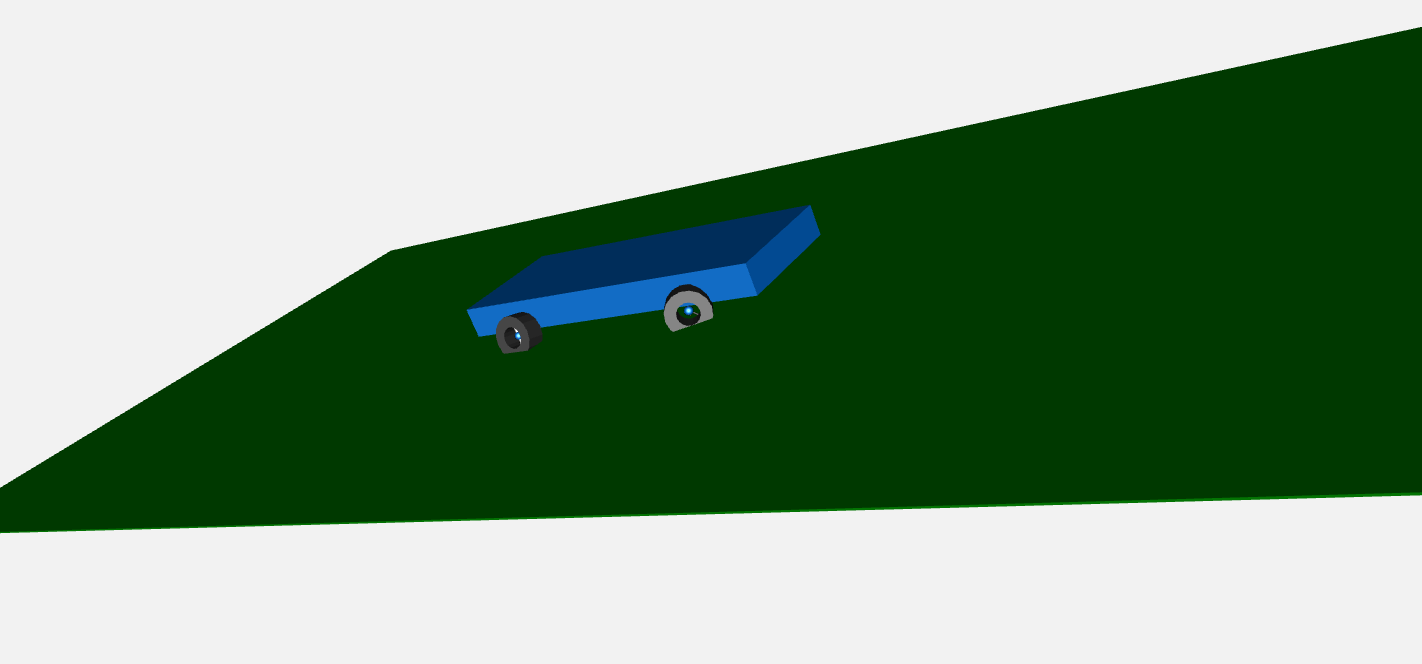
\includegraphics[width=1\textwidth]{img/bodybox.png} 
    
    \vspace{1em} % Adds spacing between image and quote
    
\caption[Representación del BodyBox en Modelica]{Representación del chasis como BodyBox dentro del visualizador de OpenModelica. Este ejemplo en particular pertenece al ejemplo \textit{E36Example} . Se puede observar un paralelepípedo al cual se le conectan las diferentes partes del sistema, como ruedas y suspensiones, y se posiciona sobre un terreno representado por $y = 1$.}
\label{fig:bodybox}
\end{figure}

\subsubsection*{Parts.Suspension}

El subpaquete \verb|Suspension| contiene los modelos que representan las diferentes geometrías de suspensión. Todos ellos extienden la clase parcial \verb|BaseSuspension|, que define la interfaz común: el conector de chasis \verb|chassisMount| (\verb|Frame_a|), el conector de rueda \verb|wheelMount| (\verb|Frame_b|), los parámetros de rigidez $k$ y amortiguamiento $d$, la masa no suspendida del buje $m_\text{hub} = 15$ kg, y el conector rotacional opcional \verb|steerInput| que se activa mediante el parámetro \verb|steerable|.\\

Se implementan tres topologías de suspensión de diferente complejidad cinemática: \verb|DoubleWishbone|, \verb|McPherson| y \verb|MultiLink|.\\

\subsubsection*{DoubleWishbone (doble triángulo).}

La suspensión de doble brazo triangular, más conocida por su nombre en inglés \verb|double wishbone|, es una de las geometrías más empleadas en vehículos de competición y alto rendimiento, tanto en el eje delantero como en el trasero. Mecánicamente, consiste en cuatro barras en el plano frontal del vehículo, cuyos eslabones son: el chasis, el brazo superior (\textit{upper A-arm}), el mangueto (\textit{knuckle}) y el brazo inferior (\textit{lower A-arm}). Cada brazo pivota en el chasis mediante una rótula o bujes de goma (modelados en Modelica como \verb|Revolute| con eje transversal $\{1,0,0\}$) y se une al mangueto en su extremo exterior mediante rótulas esféricas (los puntos de rótula superior e inferior, \textit{upper} y \textit{lower ball joints}).\\

La principal ventaja de esta topología es el control independiente de la geometría cinemática de la rueda. A diferencia de una suspensión convencional, este diseño emplea brazos de diferente longitud y con diferentes alturas de montaje en el chasis, lo que permite gestionar el cambio de caída (\textit{camber}) de la rueda durante el recorrido vertical.  El \textit{centro instantáneo de rotación} (IC) del mangueto (la intersección de las rectas que pasan por cada brazo) determina el eje alrededor del cual oscila la rueda en cada instante. Elevando el IC por encima del suelo mediante la geometría de los brazos, se obtiene una recuperación de camber que mantiene al neumático más perpendicular al suelo durante el balanceo de carrocería, maximizando el área de huella y la fuerza lateral generada en curvas rápidas.\\

En la implementación de Modelica, el bucle cinemático cerrado que forma el mecanismo de cuatro barras no puede expresarse con una cadena abierta de articulaciones y cuerpos. Para resolverlo, se utiliza el objeto \verb|JointRRR| de la biblioteca \textit{MultiBody}, que parametriza analíticamente un sistema de tres revolutes y dos barras de longitud fija. El primer revolute (\verb|frame_a|) se ubica en la rótula superior, con el brazo superior como la rama de árbol cinemático, los dos revolutos restantes, junto con sus barras asociadas, forman el cierre del bucle: la barra \verb|rRod1_ia| $= \{0, -(h_\text{sup} + h_\text{inf}), 0\}$ representa el mangueto (de longitud $h_\text{sup} + h_\text{inf} = 0{,}40$ m en la parametrización por defecto) y la barra \verb|rRod2_ib| $= \{0, 0, \pm L_\text{inf}\}$ representa el brazo inferior. Esta forma de modelar el sistema permite al compilador de OpenModelica resolver el sistema de restricciones algebraicas sin introducir multiplicaciones de Lagrange extra reduciendo el índice del DAE resultante y mejorando la estabilidad numérica \cite{otter2003}.\\

El centro de la rueda se ubica en el punto medio del mangueto, a $\frac{h_\text{sup} + h_\text{inf}}{2}$ por debajo de la rótula superior, mediante una traslación fija \verb|wheelOffset|. El amortiguador conecta un punto elevado del chasis (\verb|shockTopMount|, a 0{,}35 m sobre el montaje de la suspensión) con el punto de rótula inferior (\verb|frame_im| del \verb|JointRRR|), de manera que la fuerza del resorte actúa aproximadamente en la dirección vertical, en la región del espacio entre los dos brazos.\\

La dirección se implementa mediante un \verb|Revolute| adicional con eje vertical $\{0,1,0\}$ (eje de pivote o eje de \textit{kingpin}), interpuesto entre \verb|wheelOffset| y \verb|wheelMount|. En los ejes que permiten dirección (\verb|steerable = true|), la posición angular de este \verb|Revolute| es impuesta por el actuador \verb|steerAct|. En los ejes sin dirección, el \verb|Revolute| queda bloqueado cinemáticamente por un componente \verb|Fixed| conectado en una cláusula condicional \verb|if not steerable|, un idioma propio de Modelica que elimina físicamente el componente del sistema de ecuaciones cuando la condición no se cumple.\\

% \begin{figure}[H]
% \centering
% \begin{tikzpicture}[scale=1.25, >=Latex, font=\small,
%     piv/.style={circle, draw, fill=white, line width=0.8pt, inner sep=1.5pt},
%     bj/.style={circle, draw, fill=black, inner sep=1.5pt},
%     arm/.style={line width=1.4pt, black!75}]

%   % --- coordenadas ---
%   \coordinate (A)  at (0,2.4);      % pivote superior en el chasis
%   \coordinate (B)  at (0,1.6);      % pivote inferior en el chasis
%   \coordinate (C)  at (3.6,2.76);   % rótula superior
%   \coordinate (D)  at (4.0,0.4);    % rótula inferior
%   \coordinate (W)  at (3.8,1.58);   % centro de rueda
%   \coordinate (IC) at (-2.0,2.2);   % centro instantáneo
%   \coordinate (S)  at (0,3.2);      % anclaje superior del amortiguador
%   \coordinate (M)  at (1.6,1.12);   % anclaje inferior (sobre el brazo inferior)
%   \coordinate (P)  at (3.8,0);      % huella de contacto

%   % --- suelo ---
%   \draw[line width=1pt] (-2.6,0) -- (5.7,0);
%   \foreach \x in {-2.5,-2.2,...,5.6} \draw[black!55] (\x,0) -- ++(-0.18,-0.22);

%   % --- chasis ---
%   \fill[black!10] (-0.55,1.15) rectangle (0,3.45);
%   \draw[line width=1pt] (0,1.15) -- (0,3.45);
%   \foreach \y in {1.3,1.6,...,3.4} \draw[black!45] (-0.55,\y) -- ++(0.2,-0.18);
%   \node[anchor=south] at (-0.27,3.5) {chasis};

%   % --- construcción del centro instantáneo ---
%   \draw[dashed, black!55] (C) -- (IC);
%   \draw[dashed, black!55] (D) -- (IC);
%   \node[bj, fill=black!55, inner sep=1.3pt] at (IC) {};
%   \node[anchor=east] at (IC) {CI};

%   % --- rueda ---
%   \draw[line width=1.5pt, black!45] (W) circle (1.58);
%   \node[black!55] at (3.0,0.5) {rueda};

%   % --- muelle-amortiguador ---
%   \draw[decorate, decoration={coil, aspect=0.6, segment length=2.2mm, amplitude=1.5mm},
%         line width=0.8pt] (S) -- (M)
%         node[midway, sloped, below=1pt, font=\footnotesize]{resorte-amortiguador};

%   % --- brazos y mangueto ---
%   \draw[arm] (A) -- (C) node[midway, sloped, above=2pt]{brazo superior};
%   \draw[arm] (B) -- (D) node[midway, sloped, below=2pt]{brazo inferior};
%   \draw[arm] (C) -- (D);
%   \node[anchor=west] at (4.35,1.95) {mangueto};
%   \draw[thin] (4.33,1.95) -- (3.86,1.62);

%   % --- marcadores de articulaciones ---
%   \node[piv] at (A) {}; \node[piv] at (B) {};
%   \node[bj]  at (C) {}; \node[bj]  at (D) {};
%   \fill (W) circle (1.7pt);
%   \fill (P) circle (1.7pt); \node[anchor=north] at (3.8,-0.03) {\footnotesize huella};



% \end{tikzpicture}
\begin{figure}[htbp]
    \centering
    % Replace 'example-image' with your file name
    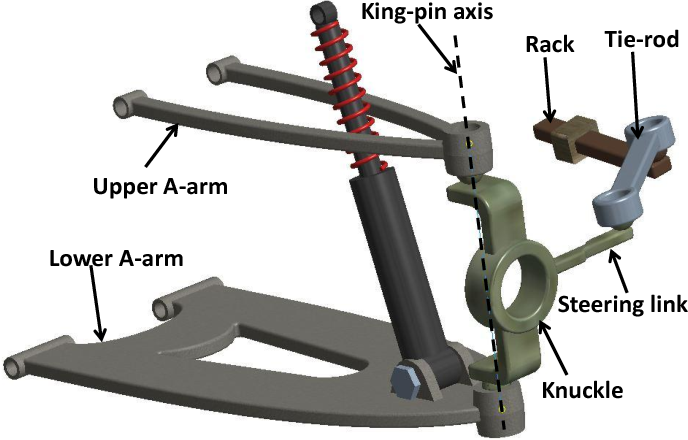
\includegraphics[width=1\textwidth]{img/double_wishbone.png} 
    
    \vspace{1em} % Adds spacing between image and quote
    

\caption[Esquema del mecanismo de doble triángulo]{Esquema cinemático de la suspensión de doble triángulo (\texttt{DoubleWishbone}) en el frontal del vehículo. El mecanismo de cuatro barras esta formado por el chasis, el brazo superior, el mangueto y el brazo inferior. El centro de la rueda se encuentra en el punto medio del mangueto. La intersección de las prolongaciones de los brazos define el centro instantáneo de rotación (IC), cuya posición controla la variación de caída durante el recorrido vertical \cite{doublewishbone}}
\label{fig:double-wishbone}
\end{figure}

\begin{figure}[htbp]
    \centering
    % Replace 'example-image' with your file name
    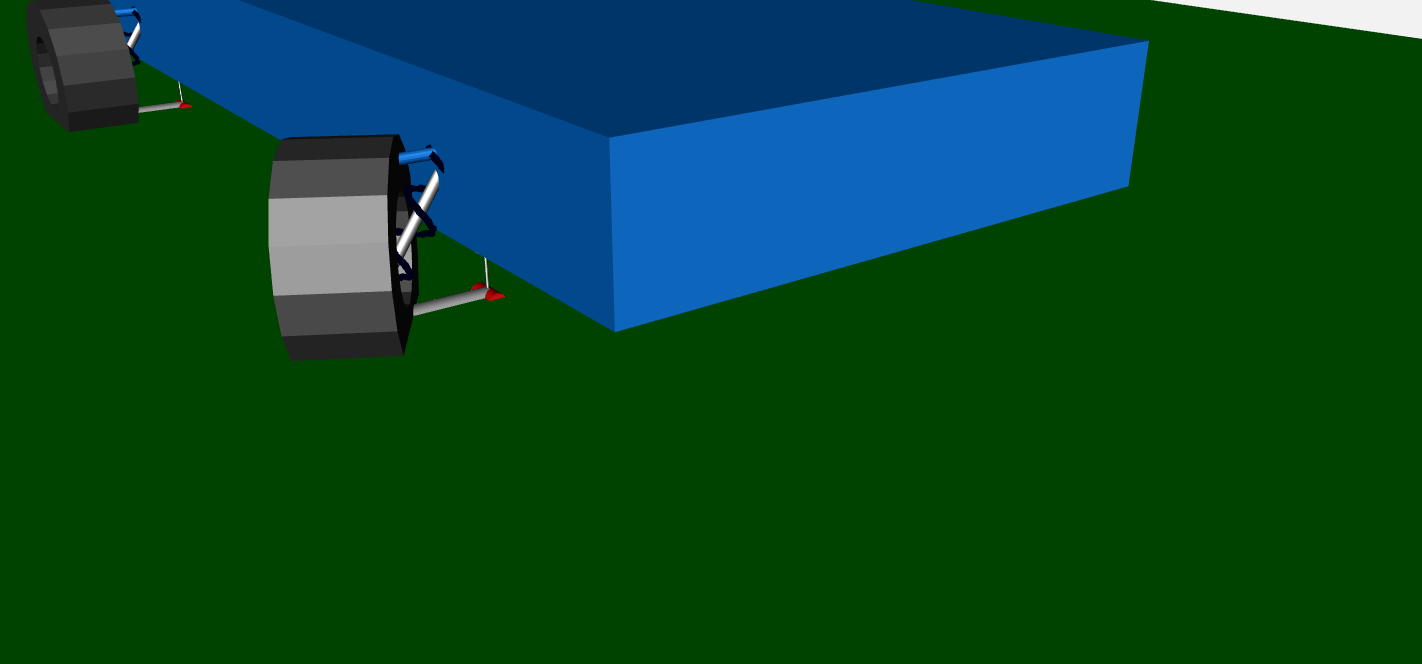
\includegraphics[width=1\textwidth]{img/doublewishbone.png} 
    
    \vspace{1em} % Adds spacing between image and quote
    
\caption[Representación de Double Wishbone en Modelica]{Representación de la geometría Double Wishbone en el visualizador de OpenModelica, con la implementación del objeto \textit{DoubleWishbone}. Esta imagen pertenece al ejemplo de \textit{CivicEKExample}, que implementa esta geometría en las cuatro puntas.}
\label{fig:doublewishbone}
\end{figure}
\newpage
\subsubsection*{McPherson (puntal telescópico).}

El puntal McPherson (\verb|McPherson Strut|) es la topología de suspensión mas utilizada en la industria automotriz de gran escala debido a su bajo coste, simplicidad constructiva y peso reducido. En un diseño real, el puntal es un elemento estructural que integra el amortiguador telescópico y la guía superior de la rueda: su extremo superior se fija a la carrocería mediante un rodamiento de apoyo que permite la rotación para la dirección, y su extremo inferior se une al mangueto (\verb|knuckle|). Un brazo inferior de triángulo (a veces conocido como parrilla) aporta la única restricción cinemática lateral, haciendo que el conjunto tenga un único grado de libertad de desplazamiento vertical. A diferencia del \verb|double wishbone|, el mangueto no tiene un punto de rótula superior independiente: el propio puntal actúa como guía rígida del mangueto, de modo que el eje de este cambia de orientación con el ángulo de dirección.\\

El modelo de esta librería, \verb|McPherson| adopta una simplificación deliberada: reemplaza el mecanismo de cinco eslabones (chasis, puntal, mangueto, brazo inferior, subchasis) por una única articulación \verb|Prismatic| de eje $\{0,-1,0\}$, que controla el desplazamiento vertical de la rueda. Esta decisión de implementación elimina el brazo inferior como restricción cinemática activa, y con ello también se pierde la variacíon de anchura de vía y de caída que aparecería en un modelo más detallado, a cambio de una mejor performance y simplicidad del modelo. Para reemplazar al brazo inferior se introduce una traslación fija \verb|knuckleOffset| que desplaza el centro de rueda respecto al extremo del puntal: \verb|wheelOffsetY| eleva el centro de rueda sobre la base del puntal (equivalente a la altura del mangueto) y \verb|wheelOffsetZ| lo desplaza lateralmente hacia el exterior (equivalente a la longitud efectiva del brazo inferior). Estos dos parámetros deben ajustarse en cada modelo de vehículo concreto para que la anchura de vía y la altura de rodaje del eje delantero sean coherentes con la geometría real del vehículo.\\

El resorte-amortiguador conecta el montaje superior fijo al chasis (\verb|shockTopMount|, elevado 0{,}28 m sobre el punto de anclaje del puntal con las configuraciones estándar) con la base del puntal (\verb|strutTravel.frame_b|). Por defecto, la longitud libre del conjunto es de 0{,}41 m, calculada geométricamente como $\sqrt{(0{,}28)^2 + (0{,}30)^2}$ para que el resorte este sin carga con el puntal a 0{,}30 m de compresión inicial. La dirección se implementa con el mismo \verb|Revolute| de eje vertical y la misma lógica condicional que en \verb|DoubleWishbone|.\\

La simplificación introducida es aceptable en el contexto de la dinámica vehicular a escala global: para la predicción del balanceo y transferencia de pesos laterales, las contribuciones de la cinemática de suspensión de primer orden son pequeñas frente a las de rigidez del resorte y la masa de la carrocería. Esta topología se emplea en el modelo \verb|E36Car| para el eje delantero, donde la limitación de espacio y la tracción trasera hacen que la variación de caída durante el giro no sea el factor limitante del comportamiento dinámico.\\

\begin{figure}[htbp]
% \centering
% \begin{tikzpicture}[scale=1.25, >=Latex, font=\small,
%     piv/.style={circle, draw, fill=white, line width=0.8pt, inner sep=1.5pt},
%     bj/.style={circle, draw, fill=black, inner sep=1.5pt},
%     arm/.style={line width=1.4pt, black!75}]

%   % --- coordenadas ---
%   \coordinate (B) at (0,0.9);       % pivote del brazo inferior en el chasis
%   \coordinate (L) at (3.1,0.55);    % rótula inferior
%   \coordinate (S) at (2.75,3.5);    % apoyo superior (cojinete a la carrocería)
%   \coordinate (Q) at (2.93,1.7);    % asiento inferior del resorte
%   \coordinate (T) at (2.95,1.55);   % unión del mangueto al puntal
%   \coordinate (W) at (3.75,1.55);   % centro de rueda
%   \coordinate (P) at (3.75,0);      % huella de contacto
%   \coordinate (G) at (3.165,0);     % eje de dirección en el suelo

%   % --- suelo ---
%   \draw[line width=1pt] (-1.4,0) -- (5.7,0);
%   \foreach \x in {-1.3,-1.0,...,5.6} \draw[black!55] (\x,0) -- ++(-0.18,-0.22);

%   % --- chasis ---
%   \fill[black!10] (-0.55,0.55) rectangle (0,2.5);
%   \draw[line width=1pt] (0,0.55) -- (0,2.5);
%   \foreach \y in {0.7,1.0,...,2.4} \draw[black!45] (-0.55,\y) -- ++(0.2,-0.18);
%   \node[anchor=south] at (-0.27,2.55) {chasis};

%   % --- eje de dirección (kingpin) hasta el suelo ---
%   \draw[dashed, black!55] (2.68,3.72) -- (G);
%   \node[anchor=east, font=\footnotesize] at (2.0,0.42) {eje de dirección};
%   \draw[thin] (2.05,0.42) -- (3.12,0.33);

%   % --- apoyo superior (cojinete a la carrocería) ---
%   \draw[line width=1pt] (2.35,3.62) -- (3.15,3.62);
%   \foreach \x in {2.4,2.6,...,3.1} \draw[black!55] (\x,3.62) -- ++(0.14,0.16);
%   \node[anchor=south, font=\footnotesize] at (2.75,3.7) {apoyo superior};

%   % --- rueda ---
%   \draw[line width=1.5pt, black!45] (W) circle (1.55);
%   \node[black!55] at (4.45,2.35) {rueda};

%   % --- puntal: resorte (coil) + vástago ---
%   \draw[decorate, decoration={coil, aspect=0.6, segment length=2.2mm, amplitude=1.6mm},
%         line width=0.8pt] (S) -- (Q);
%   \draw[arm] (Q) -- (L);
%   \node[anchor=east, align=center, font=\footnotesize] at (2.1,2.6) {puntal\\(resorte-\\amortiguador)};

%   % --- brazo inferior ---
%   \draw[arm] (B) -- (L) node[midway, sloped, below=2pt]{brazo inferior};

%   % --- mangueto / spindle ---
%   \draw[arm] (T) -- (W);
%   \node[anchor=south west, font=\footnotesize] at (3.15,1.6) {mangueto};

%   % --- marcadores de articulaciones ---
%   \node[piv] at (S) {};
%   \node[piv] at (B) {};
%   \node[bj]  at (L) {};
%   \fill (W) circle (1.7pt);
%   \fill (P) circle (1.7pt); \node[anchor=north] at (3.75,-0.03) {\footnotesize huella};

% \end{tikzpicture}
\centering
% Replace 'example-image' with your file name
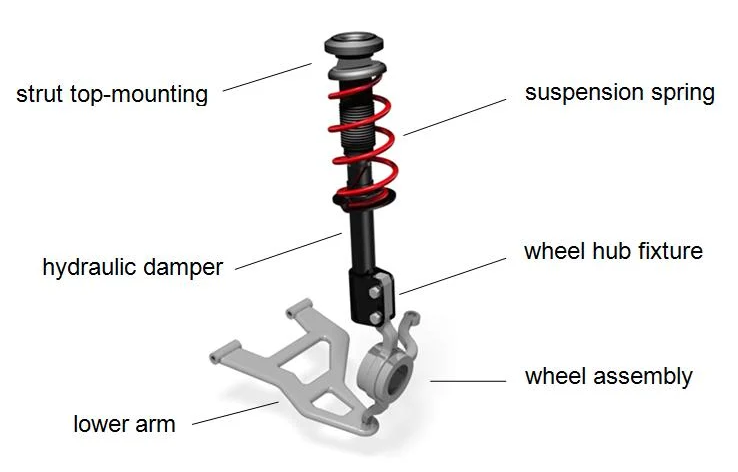
\includegraphics[width=1\textwidth]{img/mcpherson_diag.png} 

\vspace{1em} % Adds spacing between image and quote
    

\caption[Esquema del puntal McPherson]{Esquema del puntal \texttt{McPherson}. El conjunto resorte-amortiguador (puntal) es a la vez elemento elástico y guía superior de la rueda: su extremo superior se ancla a la carrocería mediante un buje que permite el giro de dirección, y su extremo inferior forma cuerpo con el mangueto. Un único brazo inferior aporta la localización lateral, con una rótula esférica  en la rueda y una articulación Revolute en el chasis. A diferencia del doble triángulo, no existe rótula superior independiente: el eje de dirección queda definido por la recta que une el apoyo superior con la rótula inferior. \cite{mchperson}}
\label{fig:mcpherson}
\end{figure}
\newpage

\subsubsection*{MultiLink (eje de vínculos múltiples).}

La suspensión multibrazo (más conocida como \textit{Multilink}) es la arquitectura de mayor complejidad cinemática de las implementadas. En un eje trasero Multilink (como el eje \textit{Z} (o \textit{Z-Axle} utilizada en el BMW E36) cada rueda está guida por cinco eslabones independientes: uno o dos brazos transversales, uno o dos brazos longitudinales y un tirante adicional \cite{reimpell2001}.  La separación de las funciones de guiado longitudinal, lateral y angular en eslabones distintos ofrece una mayor libertad de diseño comparada con otros tipos de geometría, el diseñador puede utilizar de forma casi independiente la convergencia (\textit{toe}), la caída (\textit{camber}), el avance (\textit{caster}) y la inclinación del pivote (\textit{kingpin inclination}) resultantes de cualquier combinación de desplazamiento vertical y fuerza de neumático.\\

El modelo \verb|MultiLink| implementa una versión reducida con dos eslabones transversales  (un enlace superior y un enlace inferior), conservando la topología de cuatro barras del doble triángulo pero con brazos más cortos y con el pivote del enlace inferior desplazado longitudinalmente. El cierre del bucle cinemático emplea exactamente la misma estrategia \verb|JointRRR| que \verb|DoubleWishbone|: la barra \verb|rRod1_ia| modela el mangueto y la barra \verb|rRod2_ib| modela el enlace inferior (longitud \verb|lowerLinkLength| $= 0{,}38$ m en dirección lateral).\\

% El elemento que lo diferencia de \verb|DoubleWishbone| es el parámetro \verb|rearLinkOffset|, que traslada el punto de anclaje del enlace inferior en el chasis una distancia definida (por defecto 0{,}08 m) en la dirección longitudinal $X$. Esta asimetría introduce un acoplamiento entre el desplazamiento vertical de la rueda y su ángulo de convergencia: cuando la rueda sube en compresión, el extremo interior del enlace inferior traza un arco en torno a un pivote desplazado, generando un movimiento de convergencia (\textit{toe-in}) pasivo. Este efecto (conocido como \textit{passive rear-wheel steering}) mejora la estabilidad en frenada y en la entrada a curva al aumentar la rigidez efectiva del eje ante perturbaciones laterales, sin necesitar actuadores adicionales \cite{milliken1995,reimpell2001}.  Es precisamente esta característica la que distingue al eje \textit{Z} de una simple suspensión de doble triángulo trasera.\\

% Sus dos eslabones tienen longitudes distintas, lo que genera una ganancia de caída: las dos rótulas describen arcos de radio diferente y el mangueto se va inclinando a lo largo del recorrido. Para que esa ganancia se organice alrededor de cero y no alrededor de un valor constante, el pivote del enlace inferior se sitúa más adentro que el del superior, exactamente la diferencia de longitudes (\verb|lowerLinkInboard|), con lo cual en la pose nominal ambas rótulas comparten estación lateral.\\

% La característica que lo distingue del doble triángulo, sin embargo, es la orientación del eje de articulación del varillaje. El \verb|JointRRR| obliga a que sus tres revolutos sean paralelos a un mismo eje, y el mangueto gira alrededor de ese eje a medida que la suspensión recorre. Cuando el eje es longitudinal, como en el doble triángulo, ese giro es caída y nada más. Aquí el eje está barrido un ángulo \verb|linkSweep| hacia la vertical, de $15$ grados por defecto, y el mismo giro del mangueto se reparte entonces entre caída y convergencia en la razón $\tan(\verb|linkSweep|)$. El recorrido vertical de la rueda pasa así a producir un ángulo de dirección: es la dirección pasiva de las ruedas traseras (\textit{passive rear-wheel steering}), que mejora la estabilidad en frenada y en la entrada a curva sin necesitar actuador alguno \cite{milliken1995,reimpell2001}. Se trata de la geometría de un brazo semi-arrastrado, que es de donde deriva el eje \textit{Z} del E36.\\

La característica que lo distingue del \textit{double wishbone} es la orientación del eje de articulación del varillaje. El \verb|JointRRR| fuerza a sus tres revolutes a ser paralelos y el mangueto gira alrededor de ese eje a medida de que la suspensión recorre su trayectoria. Cuando el eje es longitudinal, como en el doble triángulo, ese giro es caída y nada más. Aquí el eje está en un ángulo \verb|linkSweep| hacia la vertical, de $15$ grados por defecto y el mismo giro del mangueto se reparte entonces entre caída y convergencia. El recorrido vertical de la rueda pasa así a producir un ángulo de dirección pasiva en las ruedas traseras (\textit{passive rear-wheel steering}), que mejora la estabilidad en frenada y en la entrada a curva sin necesitar actuador alguno \cite{milliken1995,reimpell2001}. Se trata de la geometría de un brazo semi-arrastrado (\textit{semi-trailing-arm}), que es de donde deriva el eje \textit{Z} del E36. \\

El parámetro \verb|rearLinkOffset| traslada el anclaje del enlace inferior $0{,}03$ m en la dirección longitudinal $X$, de modo que el plano en el que se mueve el cuadrilátero queda inclinado hacia adelante, obteniendo $5{,}0$ grados de avance (\textit{caster}), valor representativo de un vehículo de calle.\\

Se deben aclarar las limitaciones de este modelo. En un eje multibrazo real los cinco eslabones tienen ejes de articulación no paralelos, lo que les permite prescribir convergencia, caída y avance de forma casi independiente entre sí. El objeto \verb|JointRRR| impone que los tres ejes de revolución sean paralelos, por lo que el mecanismo conserva un único grado de libertad y el reparto entre caída y convergencia queda fijado por el barrido del eje, no se pueden ajustar por separado. Esa es precisamente la limitación conocida del brazo semi-arrastrado, y no una consecuencia de la implementación.\\




% Se debe aclarar las limitaciones de este modelo: en un eje multibrazo real, los cinco eslabones tienen ejes de articulación no paralelos, lo que genera la llamada dirección pasiva de las ruedas traseras (\textit{passive rear-wheel steering}), debido al cambio dinámico del ángulo de convergencia con respecto al recorrido vertical. El ensamblaje de \verb|JointRRR| impone que los tres ejes de revolución sean paralelos entre sí, por lo que evita que el cuadrilátero pueda alterar la convergencia, que se genera con un giro del eje vertical.

% \paragraph{Lo que esta topología reducida no reproduce.} Conviene delimitar el alcance del modelo. En un eje multibrazo real —el eje \textit{Z} del BMW E36 es el caso de referencia— los cinco eslabones tienen ejes de articulación no paralelos, y es esa condición la que permite prescribir un acoplamiento entre el recorrido vertical y el ángulo de convergencia: la llamada dirección pasiva de las ruedas traseras (\textit{passive rear-wheel steering}), que mejora la estabilidad en frenada y en la entrada a curva sin requerir actuador alguno \cite{milliken1995,reimpell2001}. El ensamblaje \verb|JointRRR| impone en cambio que los tres ejes de revolución sean paralelos entre sí, lo que confina el mecanismo a un movimiento plano; y un cuadrilátero plano no puede alterar la convergencia, que es un giro alrededor del eje vertical. La medición lo verifica: la convergencia del eje trasero se mantiene en $0{,}000$ grados a lo largo de todo el recorrido. Reproducir la dirección pasiva exigiría abandonar el cierre analítico y modelar los cinco eslabones con articulaciones esféricas, a costa de introducir restricciones y variables de estado adicionales, lo que contradiría el objetivo de tiempo real que gobierna el diseño de la biblioteca. Queda por lo tanto como una simplificación asumida y no como un efecto disponible.\\


La dirección del resorte-amortiguador es análoga a la del \verb|DoubleWishbone|: desde un punto elevado del chasis (\verb|shockTopMount|, 0{,}32 m sobre el montaje) hasta el punto de rótula inferior (\verb|frame_im| del \verb|lowerLoop|). Este eje trasero no es directivo (\verb|steerable = false|), por lo que el revoluto de pivote queda bloqueado por el componente \verb|Fixed| condicional. Esto es debido a que esta geometría es utilizada en ejes traseros, por lo que normalmente no se requiere que sea direccionable.\\



\begin{figure}[htbp]
\centering
% Replace 'example-image' with your file name
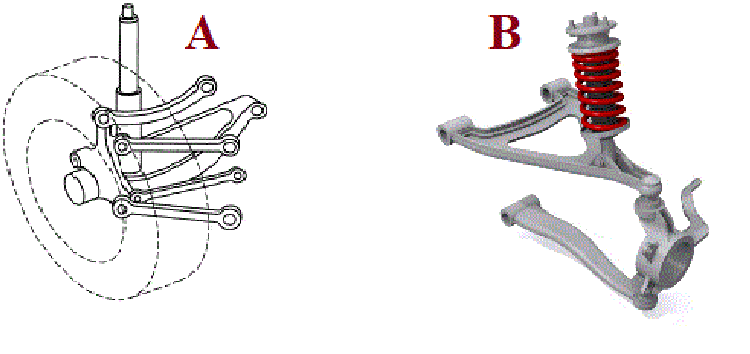
\includegraphics[width=0.8\textwidth]{img/multilink.png} 

\vspace{1em} % Adds spacing between image and quote
    

\caption[Esquema del eje MultiLink]{Esquema del eje \texttt{MultiLink}, que resalta su diferencia con respecto al doble triángulo. Los pivotes interiores del enlace superior e inferior están separados longitudinalmente una distancia \texttt{rearLinkOffset}. Esta asimetría hace que, al comprimirse la suspensión, el extremo exterior del enlace inferior describa un arco en torno a un pivote desplazado en el eje de avance, girando ligeramente el mangueto y produciendo una convergencia (\textit{toe-in}) pasiva de la rueda.\cite{multilink}}
\label{fig:multilink}
\end{figure}

\newpage

\begin{figure}[htbp]
\centering
% Replace 'example-image' with your file name
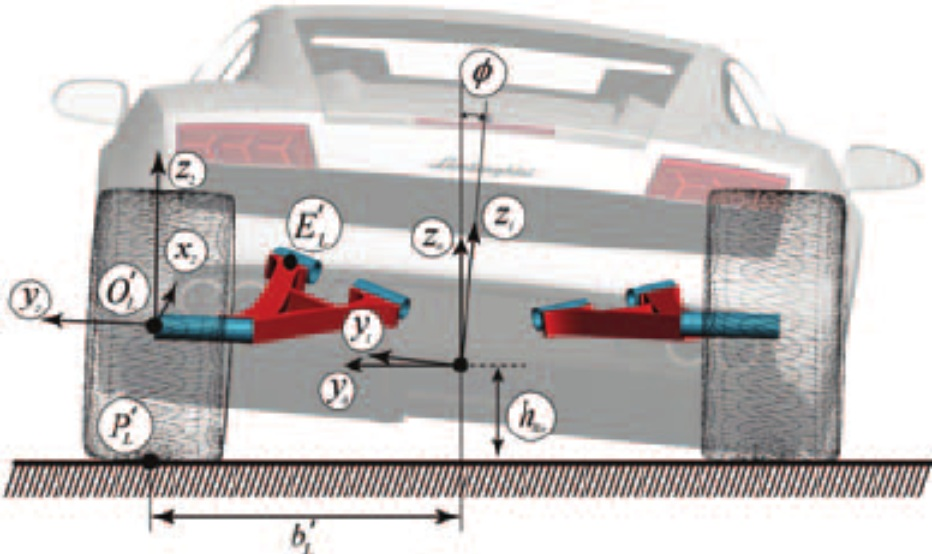
\includegraphics[width=1\textwidth]{img/trailing.jpg} 

\vspace{1em} % Adds spacing between image and quote
    

\caption[Esquema del eje MultiLink]{Esquema de la geometría \texttt{Semi-trailing-arm}, que es más cercana a la abstracción aplicada del modelo \textit{Multilink}. Se pueden apreciar como tanto la caída como la convergencia están enlazados por el mismo movimiento del recorrido de la suspensión.\cite{trailing}}
\label{fig:trailing}
\end{figure}
\newpage
\subsubsection*{Parts.RollResistance}

El subpaquete \verb|RollResistance| reúne los elementos que ayudan a la resistencia del balanceo de la carrocería. Estos elementos no afectan en el movimiento vertical del sistema. Se creó un único modelo, \verb|AntiRollBar|, que representa la barra estabilizadora en un eje.\\

Una barra estabilizadora es una barra de torsión que vincula las dos ruedas de un mismo eje. Cuando ambas ruedas recorren la misma distancia vertical, la barra gira como un cuerpo rígido, no se retuerce y no aporta rigidez, sin embargo, cuando una rueda sube y la otra baja (como por ejemplo al doblar) la barra se retuerce y aplica un par opuesto al movimiento realizado. Esto hace que se puedan montar resortes más blandos sin que el vehículo vuelque demasiado en curva.

% \paragraph{Fundamento.} Una barra estabilizadora es una barra de torsión que vincula las dos ruedas de un mismo eje a través del chasis. Cuando ambas ruedas recorren lo mismo —al pasar sobre un badén, por ejemplo— la barra gira como un cuerpo rígido, no se retuerce y no aporta rigidez alguna. Cuando en cambio una rueda sube y la otra baja, como ocurre al virar, la barra se retuerce y opone un par al movimiento diferencial. Esa selectividad es lo que la hace útil: permite montar resortes blandos, que dan una respuesta vertical cómoda, sin que el vehículo se incline en exceso en curva. Un automóvil de calle obtiene de ella una parte sustancial de su rigidez al balanceo \cite{gillespie1992}.\\

El modelo expone cuatro conectores \verb|Frame_a|: el anclaje al chasis y el montaje de rueda de cada lado. Dos sensores \verb|RelativePosition| miden la altura del centro de rueda respecto de su anclaje y el se aplica una fuerza que responde a la diferencia entre ambas alturas:

% \paragraph{Implementación.} El modelo expone cuatro conectores \verb|Frame_a|: el anclaje al chasis y el montaje de rueda de cada lado. Dos sensores \verb|RelativePosition| miden la altura de cada centro de rueda respecto de su propio anclaje, resuelta en ejes del chasis para que la referencia siga a la carrocería cuando esta balancea, y el elemento responde a la diferencia entre ambas:

\begin{equation}
    f = c_\text{arb} \cdot \frac{d_\text{izq} - d_\text{der}}{2}
    \label{eq:arb}
\end{equation}

La fuerza resultante se aplica utilizando dos elementos \verb|Forces.Force| que conectan en cada lado el anclaje al chasis y el montaje de la rueda. Se aplica una fuerza hacia abajo en la rueda más comprimida (y hacia arriba en el chasis de esa esquina) y otra opuesta en la otra rueda. \\

% La fuerza resultante se aplica hacia abajo en la rueda más comprimida y hacia arriba en la otra, mediante dos elementos \verb|Forces.Force| que abarcan, en cada lado, el anclaje al chasis y el montaje de rueda. Recurrir a un elemento de fuerza de \textit{MultiBody} en lugar de aplicar el par de fuerzas directamente sobre las ruedas no es una cuestión de estilo: el elemento reparte por sí mismo la reacción sobre el marco de origen, con lo cual el conjunto queda en equilibrio. Aplicar únicamente las dos fuerzas sobre las ruedas dejaría sobre el vehículo un par de balanceo externo sin reacción, que le haría ganar cantidad de movimiento angular sin causa física.\\

% \paragraph{Propiedades.} En recorrido simétrico la diferencia de la Ecuación~\ref{eq:arb} se anula y la barra no interviene en absoluto, de modo que las frecuencias verticales del vehículo quedan intactas y su efecto se limita al balanceo. La ley es además puramente algebraica, por lo que el elemento agrega ecuaciones pero no estados continuos y no incrementa el tamaño del vector que el integrador debe resolver, consideración que pesa en un modelo destinado a ejecutarse en tiempo real. El parámetro \verb|c_arb| expresa la rigidez de la barra referida a la rueda, en N/m; su valor por defecto es nulo, lo que la deja inactiva.\\

Los tres vehículos fueron equipados con barras en ambos ejes. El monoplaza lleva $13$ kN/m en cada uno, el E36, $31$ kN/m adelante y $16$ kN/m atrás, el Civic, $41$ y $23$ kN/m. En los dos vehículos de calle el reparto es delantero, disposición habitual para favorecer el subviraje en el límite, lo que lleva a una mayor seguridad en el manejo.\\


\subsubsection*{Parts.Tires}

El subpaquete \verb|Tires| se encarga de modelar los neumáticos como cuerpos rígidos con masa $m_\text{tire} = 20$ kg (por defecto) conectados a la suspensión mediante un \verb|Revolute| de giro libre, se implementaron dos variantes:

\begin{itemize}
    
    \item \verb|Tire|: Neumático pasivo. El \verb|Revolute| que se encarga del giro tiene su brida de eje expuesta como \verb|brakeFlange| (\verb|flange_b|) para la conexión del freno, pero no recibe par motor, representa una rueda no traccionada.
    
    \item \verb|DrivingTire|: Neumático motriz. El modelo es idéntico a \verb|Tire|, pero añade un conector \verb|spinInput| (\verb|Flange_a|) que recibe el par de torque del diferencial. La brida de freno (\verb|brakeFlange|) y la de tracción (\verb|spinInput|) se comparten sobre el mismo eje del \verb|Revolute|, de modo que el par neto aplicado es la suma algebraica de ambas contribuciones.
\end{itemize}

El subcomponente \verb|TireVisualizer| renderiza cada neumático, copiando el objeto de la librería \textit{Visualizers} de \textit{MultiBody} \verb|MultiBody.Visualizers.VoluminousWheel|, esta se encarga de generar un toroide para la forma del neumático en sí y un cilindro hueco que representa la llanta, ambos parametrizados con el radio \verb|rTire| propagado desde el nivel de ejemplo mediante \texttt{outer}. El único cambio que se le aplicó a la clase original fueron cambios de coordenadas y orientaciones para que sigan un recorrido fiel al modelo que se está simulando.\\

\begin{figure}[htbp]
    \centering
    % Replace 'example-image' with your file name
    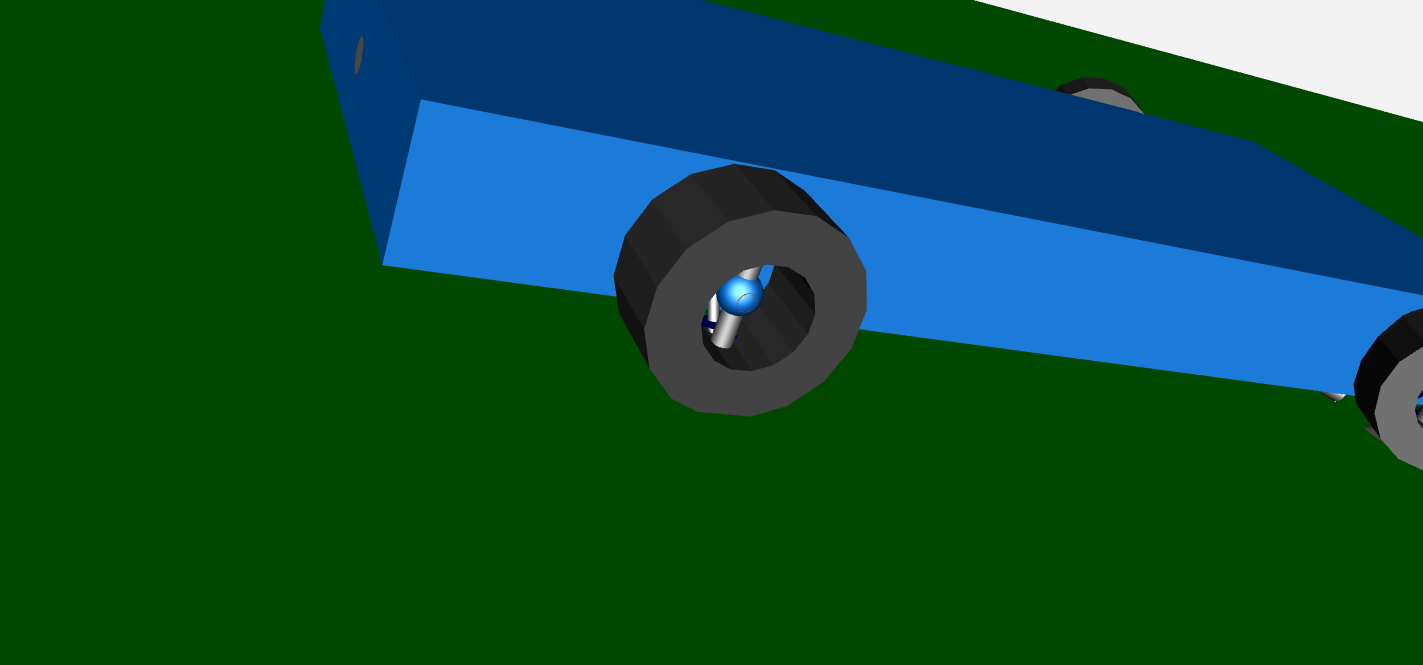
\includegraphics[width=1\textwidth]{img/tire.png} 
    
    \vspace{1em} % Adds spacing between image and quote
    
\caption[Representación de Tire en Modelica]{Representación de una rueda utilizando el objeto \textit{Tire} dentro del visualizador de OpenModelica, la geometría es generada por el componente \textit{TireVisualizer}. Esta imágen fue capturada del ejemplo \textit{CivicEKExample}, la rueda está conectada al chasis mediante una geometría de suspensión Double Wishbone}
\label{fig:tire}
\end{figure}

\subsubsection*{Parts.Differentials}

El subpaquete \verb|Differentials| modela el componente que se encarga de transmitir el par proveniente de la transmisión a las ruedas. La clase parcial \verb|Differential| define únicamente la interfaz mecánica común: una brida rotacional de entrada de par \verb|pedalInput| (\verb|Flange_a|), alimentada por la transmisión, y dos bridas rotacionales de salida hacia las ruedas (\verb|left_out| y \verb|right_out|). No contiene ecuaciones, ya que es cada subclase concreta la que decide cómo el par se distribuye en las dos ruedas.\\

\subsubsection*{Eje rígido}

Un eje rígido (\textit{solid axle} o \textit{live axle}) conecta mecánicamente ambas ruedas del mismo eje mediante semiejes que giran necesariamente a la misma velocidad angular. Esta arquitectura es la más sencilla posible desde el punto de vista constructivo, tiene consecuencias directas en el comportamiento en la curva, al doblar, la rueda exterior debe recorrer un arco de mayor radio que la interior y, por lo tanto debería girar más rápido, pero, al estar ambas ruedas girando a la misma velocidad, esta diferencia de velocidad se absorbe mediante deslizamiento lateral de los neumáticos (\textit{tire scrub}), lo que genera calor, desgaste y una tendencia al sobreviraje en curvas cerradas. En lo que respecta a la dinámica del vehículo, el eje rígido introduce un acoplamiento entre el movimiento de guiñada (\textit{yaw}) del chasis y el estado de tracción de ambas ruedas: en una curva cerrada con aceleración, la rueda interior tiende a patinar antes que la exterior, ya que recibe el mismo par pero con menor carga, comportamiento característico del vehículo de tracción trasera con eje sólido. Este tipo de eje es muy común en kartings debido a su simplicidad de mantenimiento. \\

\paragraph{Implementación como nodo mecánico de par.}

A diferencia de un enfoque basado en una restricción cinemática de velocidad, que forzaría ambas ruedas a igual velocidad, pero que introduciría un lazo algebraico de índice elevado e impediría que el par de frenado modificara la velocidad de las ruedas motrices, \verb|SolidAxle| se implementa como un simple nodo mecánico: conecta la brida de entrada \verb|pedalInput| directamente a ambas salidas \verb|left_out| y \verb|right_out|, de modo que la transmisión y las dos ruedas comparten un único nodo rotacional:

\begin{equation}
    \varphi_\text{ped} = \varphi_\text{izq} = \varphi_\text{der}
\end{equation}

Ambas ruedas traseras giran a la misma velocidad angular, sin acción diferencial de velocidad, como corresponde a un eje bloqueado, y el par entregado por la transmisión se distribuye mecanicamente a través de ese nodo hacia las ruedas, en vez de ser forzado por una fuente interna. El modelo no tiene parámetros propios: el esfuerzo motor se fija en la transmisión (parámetro \verb|torqueValue| de \verb|MockTransmission|).\\

La ventaja de modelar el diferencial mediante intercambio de par radica en la interacción entre este y el freno. Como todos los conectores son bridas rotacionales (\verb|Flange|), cualquier par aplicado sobre las bridas de las ruedas se suma sobre el nodo compartido, de manera que el par aplicado por un objeto \verb|DiscBrake| sobre una rueda se resta directamente del par motor y desacelera el eje, como lo haría un freno real, sin necesidad de vencer ninguna restricción cinemática. La velocidad resultante de las ruedas no se impone, si no que emerge naturalmente del par motor, el de frenado, la inerciad e las ruedas y las fuerzas de contacto con el suelo. Esta clase se podría extender agregando un diferencial abierto o uno autoblocante encaminando el par de entrada a través de un \verb|IdealPlanetary| o de ecuaciones de reparto de par que permitan una diferencia de velocidad entre las dos ruedas.\\

\subsubsection*{Parts.Brakes}

El modelo \verb|DiscBrake| modela el comportamiento de un freno de disco, aplicando par a la brida rotacional de cada neumático.\\

\subsubsection*{DiscBrake}

En un freno a disco real, una pinza hidráulica aprieta dos pastillas de fricción contra ambas caras de un disco conectado al eje de la rueda. La fuerza de contacto normal $N$ es proporcional a la presión hidráulica del circuito de frenos, que a su vez es función de la fuerza ejercida por el conductor sobre el pedal. El par de frenado resultante sigue el modelo de fricción de Coulomb es proporcional a la fuerza normal y al coeficiente de fricción de las pastillas $\mu_p$, y actúa siempre en sentido opuesto a la rotación de la rueda \cite{rajamani2012}:

\begin{equation}
    \tau_\text{Coulomb} = -\mu_p \cdot N_{max} \cdot r_\text{eff} \cdot \text{sign}(\omega)
\end{equation}

donde $r_\text{eff}$ es el radio efectivo medio del disco. En el modelo \verb|DiscBrake|, el producto $\mu_p \cdot N_\text{max} \cdot r_\text{eff}$ queda parametrizado directamente como \verb|maxBrakeTorque| $= \tau_\text{max}$, y la demanda normalizada $u \in [0, 1]$ escala la fuerza normal, reproduciendo la relación entre la posición del pedal y el par generado:

\begin{equation}
    \tau_\text{ideal} = -u \cdot \tau_\text{max} \cdot \text{sign}(\omega)
\end{equation}

Los valores de \verb|maxBrakeTorque| asignados a los distintos vehículos de la biblioteca —2000 N$\cdot$m para el modelo genérico, 2500 N$\cdot$m en el eje delantero del E36 y 3000 N$\cdot$m en el trasero, son coherentes con los rangos de par de frenado de vehículos de turismo de producción \cite{rajamani2012}.\\

% \paragraph{El problema de la discontinuidad y la regularización \textit{tanh}.}

La función $\text{sign}(\omega)$  presenta una discontinuidad en $\omega = 0$ que tiene consecuencias graves para la integración numérica: en los solucionadores DAE de paso variable, toda discontinuidad activa un mecanismo de detección de cruce por cero (\textit{zero-crossing detection}) que obliga a reducir el paso de integración y relanzar el solver desde el instante del evento \cite{armstrong1994}. En un modelo de vehículo con cuatro frenos activos, esto puede disparar eventos múltiples y sincronizados que afectan de manera significativamente negativa al rendimiento en tiempo real. Adicionalmente, cuando la velocidad angular oscila en torno a cero (rueda próxima a bloqueo), la función signo puede provocar alternancia rápida de signo del par (chattering) que excita modos de alta frecuencia numéricamente.\\

Para resolver este problema, el modelo reemplaza la función signo por una tangente hiperbólica regularizada:

\begin{equation}
    \tau_\text{freno} = -u \cdot \tau_\text{max} \cdot \tanh\!\left(k_s \cdot \omega\right)
\end{equation}

La función $\tanh(k_s \cdot \omega)$ es $C^\infty$ en todo $\mathbb{R}$ y reproduce el comportamiento de Coulomb fuera de la zona de transición. Para analizarla, se distinguen dos regímenes según el valor de $k_s \cdot |\omega|$:

\begin{itemize}
    \item \textbf{Régimen lineal} ($k_s \cdot |\omega| \ll 1$): $\tanh(k_s\omega) \approx k_s\omega$, de modo que el freno se comporta como un amortiguador viscoso de coeficiente efectivo $u \cdot \tau_\text{max} \cdot k_s$. En este régimen, el par es proporcional a la velocidad y el sistema no tiene discontinuidades.
    \item \textbf{Régimen de Coulomb} ($k_s \cdot |\omega| \gg 1$): $\tanh(k_s\omega) \approx \pm 1$, y el freno se aproxima al modelo ideal de Coulomb con par constante $\pm u \cdot \tau_\text{max}$.
\end{itemize}

La transición entre ambos regímenes ocurre en la zona $|\omega| \approx 1/k_s$. Con $k_s = 10$ rad$^{-1}{\cdot}$s, esta zona tiene un ancho de $\pm 0{,}1$ rad/s, equivalente a aproximadamente $\pm 1$ rpm para una rueda típica. A velocidades superiores a este umbral, el freno se comporta esencialmente como el modelo de Coulomb ideal, por debajo de él, la transición suave evita cualquier evento de cruce por cero y garantiza la continuidad diferenciable del sistema \cite{armstrong1994}. Este compromiso es adecuado para la simulación de dinámica vehicular, donde el bloqueo total de una rueda es un fenómeno de interés pero la oscilación subsecuente en torno a $\omega = 0$ no lo es.\\

\subsubsection*{Parts.Transmission}


El subpaquete \verb|Transmission| abstrae la generación del par motor hacia el diferencial a partir del input de acelerador del conductor. Sigue el mismo patrón de clase parcial que el resto de la biblioteca: \verb|BaseTransmission| define la interfaz común de una entrada \verb|pedalInput| (\verb|RealInput|) con el valor normalizado del acelerador y una salida rotacional \verb|torqueOut| (\verb|Flange_a|) que entrega el par mecánico, de modo que cualquier implementación puede sustituirse sin modificar los componentes que interactúan con este objeto (diferencial, interfaz de acelerador). Este objeto ahora mismo actúa como una combinación de motor y transmisión, así que una implementación verdadera debería modelar ambos componentes.\\

Como se mencionó anteriormente, la implementación concreta \verb|MockTransmission| es una simplificación de un conjunto de motor-transmisión, que convierte el comando del pedal en par mediante una relación lineal directa:

\begin{equation}
    \tau_\text{motor} = k_\tau \cdot u_\text{pedal}
\end{equation}

donde $k_\tau$ (representado como el parámetro \verb|torqueValue|) es el par entregado a las ruedas cuando el acelerador está a fondo y  $u_\text{pedal} \in [0, 1]$ es el input normalizado. \\ 
El par se aplica a través de una fuente \verb|Modelica.Mechanics.Rotational.Sources.Torque| y fluye por una brida \verb|torqueOut| hacia el diferencial. Para simplificar, en esta implementación, el par es constante, no tiene una retroalimentación de velocidad, por lo que el vehículo acelera hasta que la tracción y las resistencias al avance lo equilibran. Al exponer una brida portadora de par, un modelo de motor realista, con mapa de par en función del régimen, inercia del volante de inercia y relaciones de cambio, puede reemplazar a \verb|MockTransmission| conservando la misma interfaz de \verb|BaseTransmission|.\\


\subsubsection*{Parts.Steering}

De la misma forma que el paquete anterior, \verb|Steering| abstrae la conversión del comando de volante en un ángulo de giro en las ruedas. La clase parcial \verb|BaseSteering| define la interfaz como una entrada \verb|steerCmd| (\verb|RealInput|) con el comando normalizado en $[-1, 1]$ y una salida \verb|steerAngle| (\verb|RealOutput|) con el ángulo de rueda resultante, en radianes.\\

La implementación \verb|MockSteering| aplica un mapeo lineal entre ambos:

\begin{equation}
    \delta = \delta_\text{max} \cdot u_\text{steer}
\end{equation}

donde $\delta_\text{max}$ (representado por el parámetro \verb|maxSteerAngle|, con valor por defecto $0{,}53$ rad $\approx 30°$) es el ángulo de rueda cuando el volante esta al máximo de su giro y $u_\text{steer} = 0$ corresponde a la marcha recta. La salida \verb|steerAngle| se conecta a los actuadores de posición (\verb|Rotational.Sources.Position|) de las dos ruedas delanteras que reciben el mismo ángulo, ya que no se está modelando la dinámica de la columna de dirección, la relación de dirección variable ni la geometría de Ackermann. Como en el caso de la transmisión, la separación de la interfaz permite sustituir \verb|MockSteering| por un modelo más detallado sin alterar el resto del vehículo.\\

\subsection{Examples}

El paquete\verb|Examples| compila los modelos ejecutables de alto nivel: los puntos de entrada de la simulación que ensamblan un vehículo completo, el entorno y los comandos del conductor en un sistema autocontenido y simulable. Cumplen una doble función, como escenarios de validación del comportamiento dinámico y como plantillas a partir de las cuales construir nuevas simulaciones.\\


Todos los ejemplos comparten la misma estructura de ensamblaje. En primer lugar, declaran el radio de rueda como un parámetro global \\ \verb|inner parameter Real R_wheel|, que se propaga por el mecanismo \texttt{inner}/\texttt{outer} a los neumáticos y a los modelos de contacto con el suelo. A continuación instancian tres bloques principales: un vehículo (\verb|Car|, \verb|CivicEKCar| o \verb|E36Car|), el entorno \verb|Roads.Road|, que a su vez posee el \verb|World|, el terreno y los cuatro contactos de rueda, y un conjunto de fuentes de señal que emulan las acciones del conductor. Estas fuentes se conectan a las entradas normalizadas \verb|throttleInput|, \verb|steerInput| y \verb|brakeInput| del vehículo, mientras que los cuatro conectores \verb|frame_FL/FR/RL/RR| del vehículo se acoplan a los del entorno, cerrando el contacto rueda-suelo.\\

La biblioteca incluye cuatro ejemplos:

\begin{center}
\begin{tabular}{llll}
\hline
\textbf{Ejemplo} & \textbf{Vehículo} & \textbf{$R$ (m)} & \textbf{Entradas del conductor} \\
\hline
\verb|CarExample|    & \verb|Car| (Formula Ford)   & 0{,}25 & acelerador y dirección constantes,\\ & & & freno escalón en $t=3$ s \\
\verb|CivicEKExample| & \verb|CivicEKCar| (Civic EK) & 0{,}30 & acelerador y dirección constantes,\\ & & & freno escalón en $t=5$ s \\
\verb|E36Example|     & \verb|E36Car| (BMW E36)      & 0{,}31 & acelerador y dirección constantes,\\& & & freno escalón en $t=5$ s \\
\verb|CarExampleUDP|  & \verb|Car|                  & 0{,}25 & acelerador constante,\\& & & dirección sinusoidal, sin freno \\
\hline
\end{tabular}
\end{center}

Los tres primeros (\verb|CarExample|, \verb|CivicEKExample| y \verb|E36Example|) son escenarios de validación de lazo abierto, ya que aplican un input de acelerador constante y un ángulo de dirección fijo sobre un terreno plano, con una aplicación de freno luego de un tiempo determinado que permite ver la transferencia de carga longitudinal y la desaceleración del tren motriz. Se diferencian en el modelo de vehículo que se instancia, cada uno parametrizado a partir de automóviles reales de arquitectura distinta:

\begin{itemize}
    
    \item \verb|CarExample| simula el modelo \verb|Car|, inspirado levemente en un monoplaza ligero tipo Formula Ford 1600. Es el más liviano y de geometría más simétrica: chasis de 400 kg con dimensiones $3{,}0 \times 1{,}8 \times 0{,}5$ m, batalla de 3{,}0 m y vía de 1{,}8 m. Utiliza suspensión \verb|DoubleWishbone| en las cuatro puntas, con la rigidez y amortiguamiento por defecto de \verb|BaseSuspension| ($k = 30$ kN/m, $d = 2500$ N$\cdot$s/m). Es un vehículo de tracción trasera, con neumáticos \verb|DrivingTire| detrás y \verb|Tire| pasivos delante, de radio $R = 0{,}25$ m. El chasis arranca suspendido a 1{,}2 m sobre el terreno y cae hasta el equilibrio estático.
    \newpage
\begin{figure}[htbp]
    \centering
    % Replace 'example-image' with your file name
    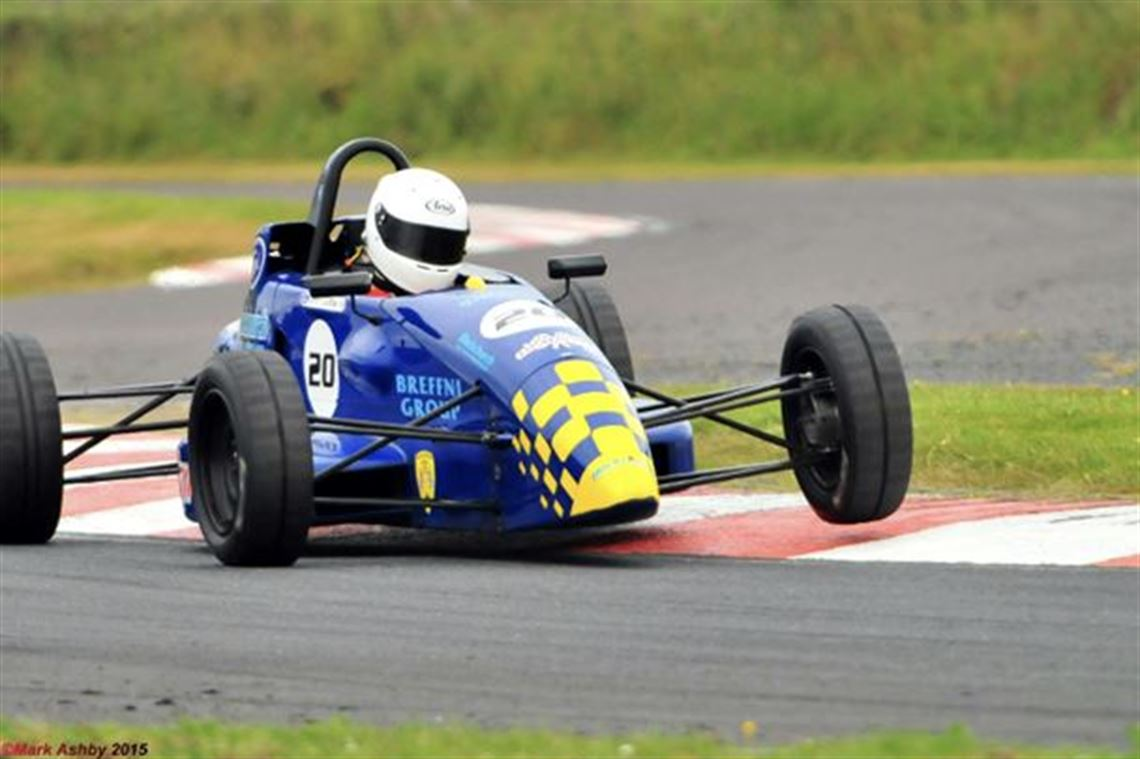
\includegraphics[width=1\textwidth]{img/fford.jpg} 
    
    \vspace{1em} % Adds spacing between image and quote
    
\caption[Formula Ford 1600]{Imágen de un vehículo Formula Ford 1600. Se puede observar las geometría de suspensión \textit{Double Wishbone}. Fuente: https://racecarsdirect.com/Advert/Details/91965/o5-ray-formula-ford-1600.}
\label{fig:ff1600}
\end{figure}

    \item \verb|CivicEKExample| simula el \verb|CivicEKCar|, basado en un Honda Civic EK hatchback de tracción delantera. Chasis de 990 kg de peso y dimensiones $4{,}178 \times 1{,}704 \times 0{,}4$ m, con batalla de 2{,}62 m y vía de 1{,}47 m. Emplea \verb|DoubleWishbone| en las cuatro esquinas, con rigidez diferenciada por eje, 16 kN/m delante y 14 kN/m detrás, y amortiguamiento de 1800 N$\cdot$s/m en las cuatro ruedas. La tracción es delantera (\verb|DrivingTire| en el eje delantero, \verb|Tire| pasivos detrás) y los neumáticos son 185/65R14 ($R = 0{,}30$ m).
\newpage
\begin{figure}[htbp]
    \centering
    % Replace 'example-image' with your file name
    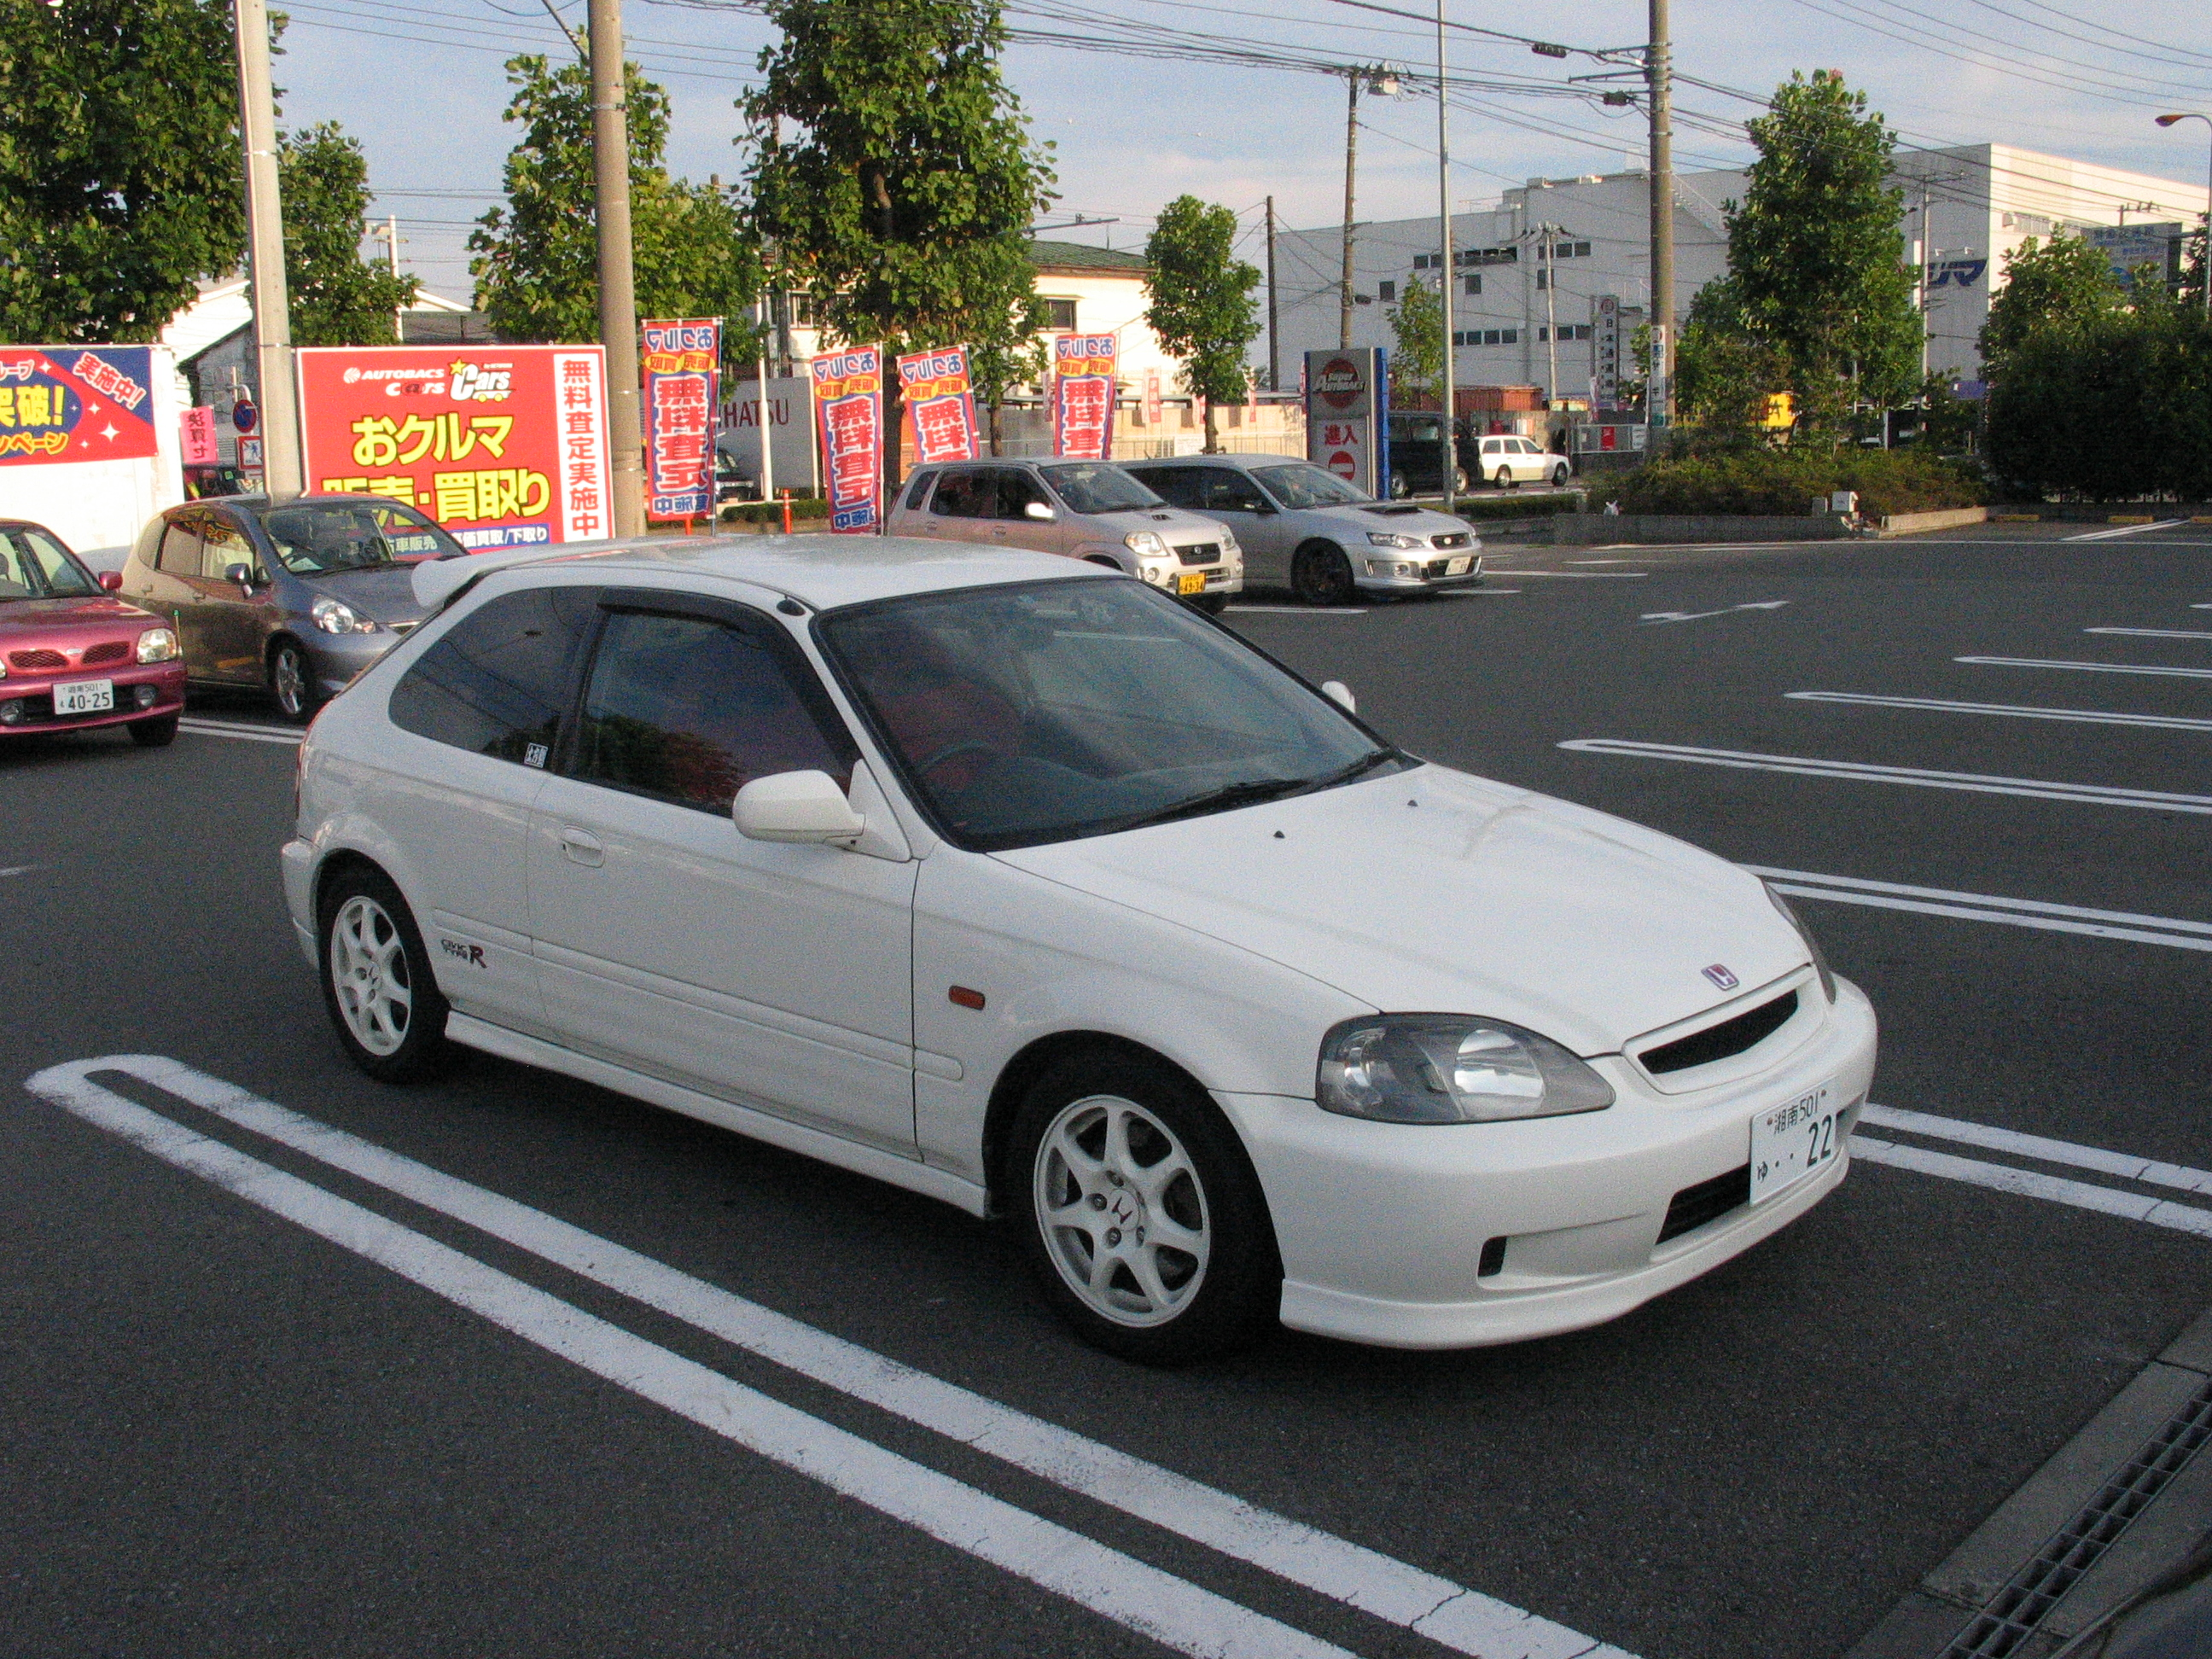
\includegraphics[width=1\textwidth]{img/civicek.jpg} 
    
    \vspace{1em} % Adds spacing between image and quote
    
\caption[Honda Civic EK]{Imágen de un vehículo Honda Civic de la generación EK. Fuente: https://es.wikipedia.org/wiki/Honda\_Civic\_(sexta\_generación).}
\label{fig:civicek}
\end{figure}
    
    \item \verb|E36Example| simula el \verb|E36Car|, basado en un BMW E36 de tracción trasera. Chasis de 1000 kg de masa suspendida y dimensiones $4{,}433 \times 1{,}710 \times 0{,}4$ m, con batalla de 2{,}70 m y vía de 1{,}42 m. Es el vehículo de geometría de suspensión más elaborada: puntal \verb|McPherson| en el eje delantero (20 kN/m, 2200 N$\cdot$s/m, con desplazamientos de mangueto \verb|wheelOffsetY| $= 0{,}25$ m y \verb|wheelOffsetZ| $= 0{,}30$ m para restituir la vía y la altura del centro de rueda) y eje trasero \verb|MultiLink| de tipo Z (16 kN/m, 2200 N$\cdot$s/m), con \verb|DrivingTire| en el eje trasero. Los neumáticos son 195/65R15 ($R = 0{,}31$ m).
\newpage
\begin{figure}[htbp]
    \centering
    % Replace 'example-image' with your file name
    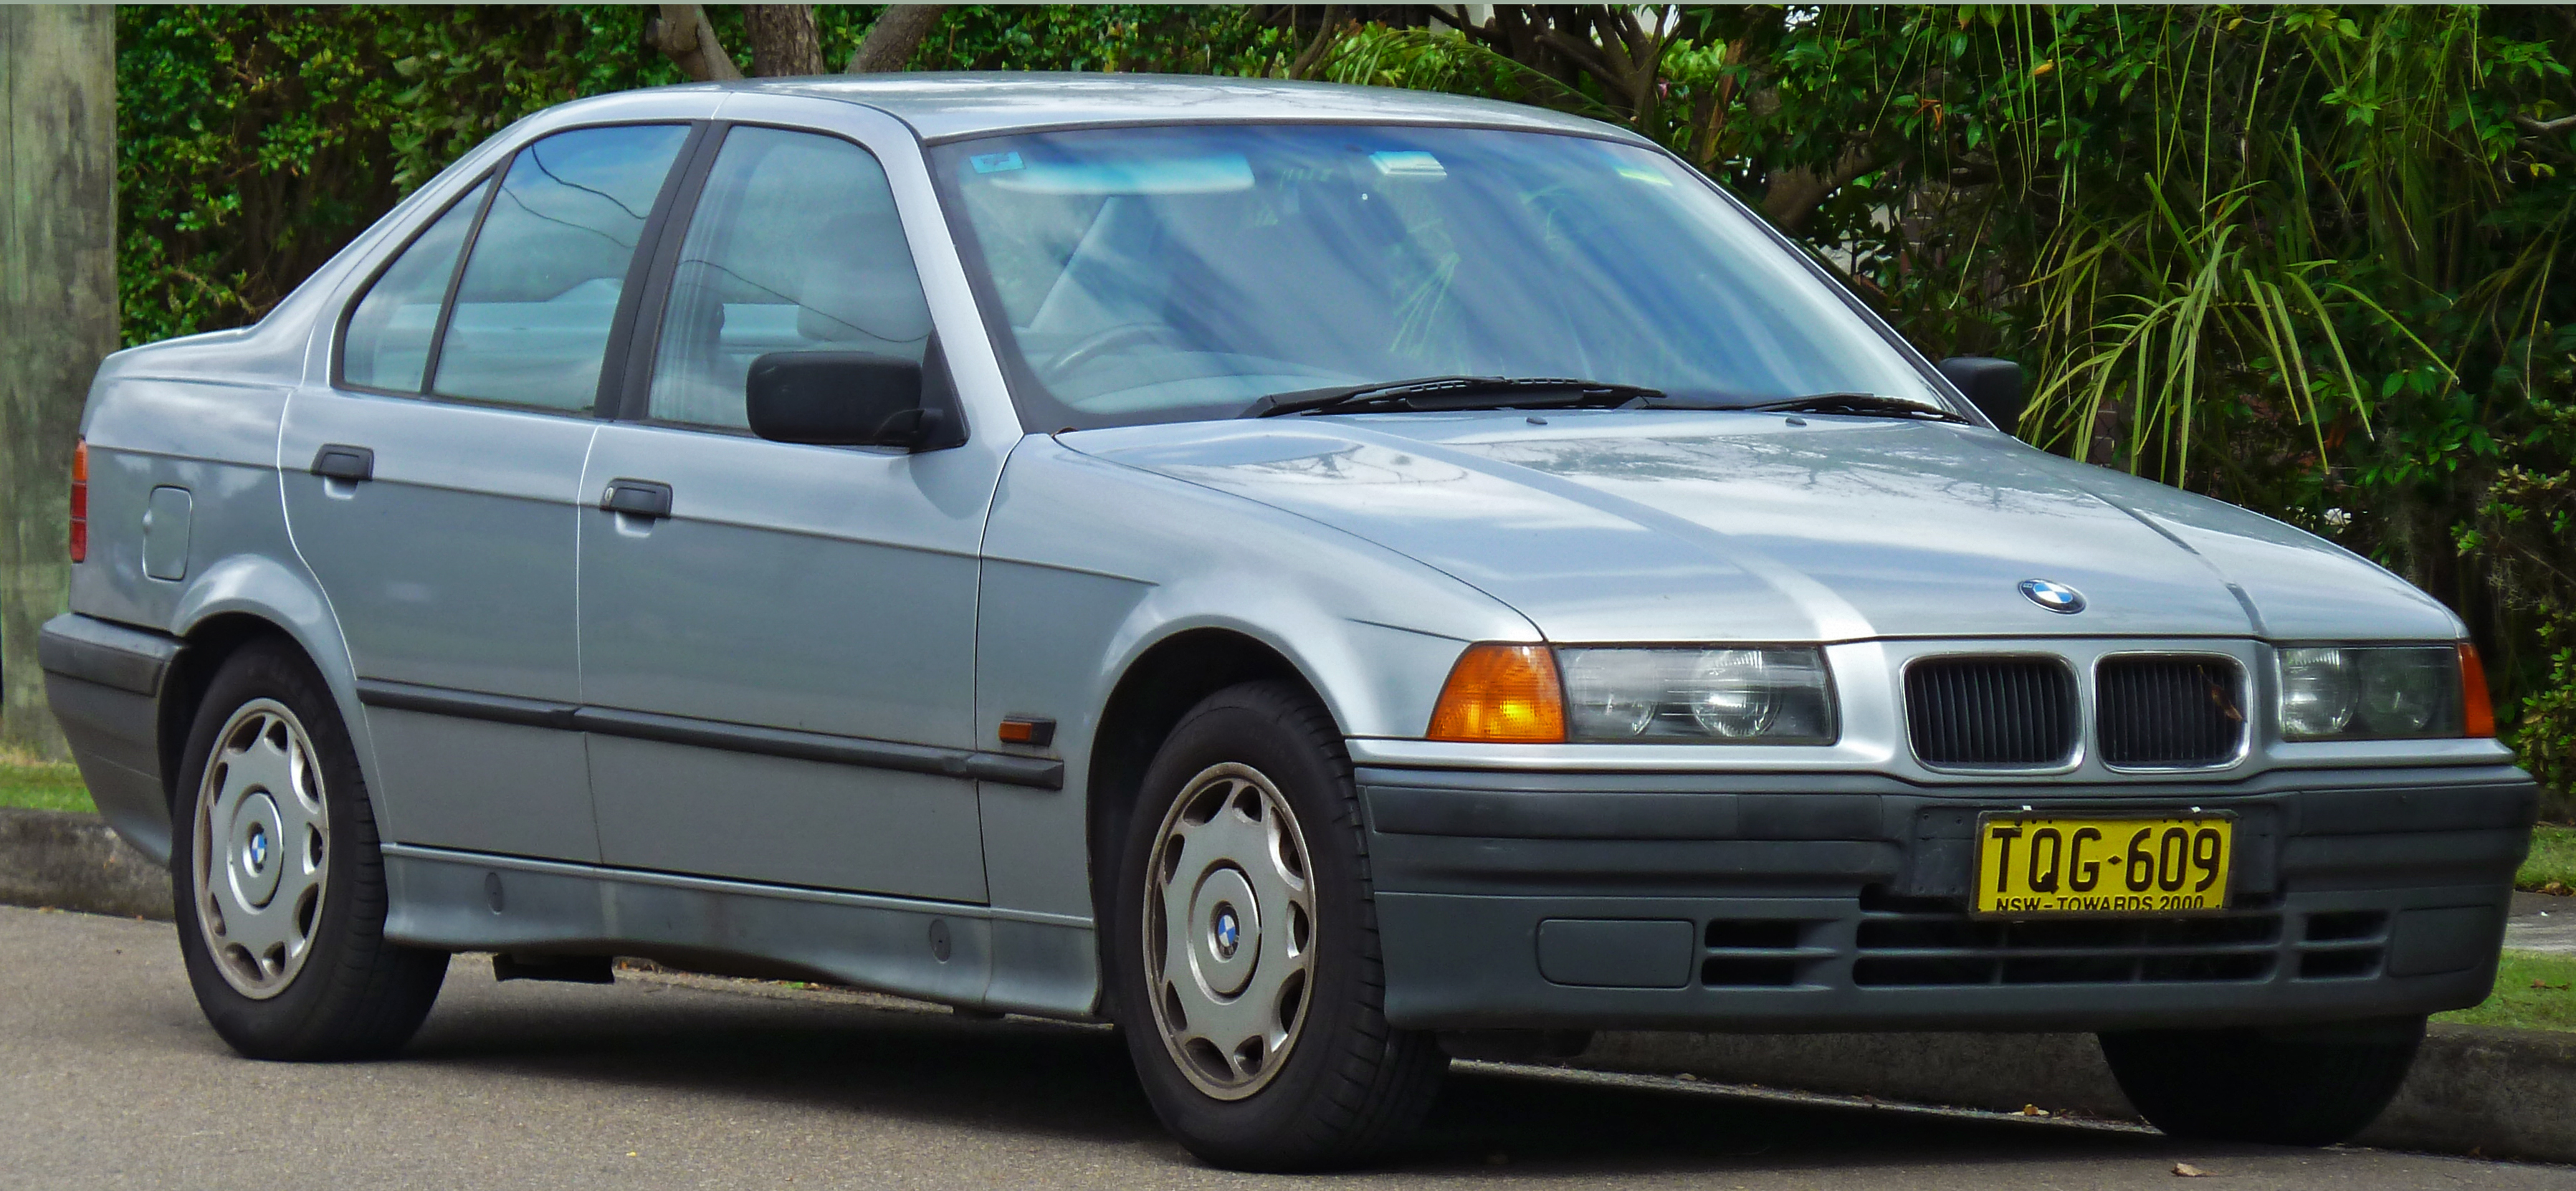
\includegraphics[width=1\textwidth]{img/e36.jpg} 
    
    \vspace{1em} % Adds spacing between image and quote
    
\caption[BMW Serie 3 E36]{Imágen de un vehículo BMW Serie 3 de la generación E36. Fuente: https://en.wikipedia.org/wiki/BMW\_3\_Series\_(E36).}
\label{fig:e36}
\end{figure}
    
\end{itemize}

Esta correspondencia (un mismo escenario de conducción aplicado a tres vehículos de masa, batalla y arquitectura de suspensión marcadamente distintas) es una demostración directa de la capacidad de reutilización que habilita el diseño modular de la biblioteca: simular un monoplaza de tracción trasera, a un hatchback de tracción delantera, o un sedan con puntal McPherson y eje multibrazo requiere solamente reemplazar el modelo del vehículo instanciado, sin alterar el entorno ni la estructura de la simulación.\\

El cuarto ejemplo, \verb|CarExampleUDP| está orientado a demostrar la visualización en tiempo real, utilizando un motor externo. Reutiliza el mismo \verb|Car| que \verb|CarExample|, pero añade cinco transmisores \verb|FrameToUDPOrientation|, uno para el chasis y uno por cada rueda, que emiten la pose completa (posición y orientación) a puertos UDP consecutivos del 12345 al 12349, de modo que un cliente en Unity (o cualquier otro visualizador) pueda renderizar elementos gráficos utilizando esta información en tiempo real. La señal de dirección es sinusoidal, para que el barrido de las ruedas pueda verificarse visualmente en el entorno gráfico. Debido a que los transmisores son sensores puros (no imponen fuerza y/o torque sobre los frames que leen), no alteran la dinámica del vehículo, y como los marcos de las ruedas se ubican sobre la salida de la junta de rotación, la orientación transmitida captura tanto el ángulo de dirección como el giro propio de cada rueda.\\


\subsection{CarExport}

El subpaquete \verb|Examples.CarExport| contiene los modelos de los tres vehículos listos para ser exportados y ejecutados desde un aplicación externa. Se diferencian de los otros ejemplos en el hecho de que no incorporan fuentes de señal, si no que exponen los comandos de entrada como inputs del modelo, para que un programa externo que gobierne la simulación los provea. Estos modelos son los que se exportan como FMU y los que usa la arquitectura de co-simulación descrita en la sección~\ref{sec:cosim}.\\

Los tres usan la clase parcial \verb|ExportInterface|, que declara la interfaz y no contiene ecuación alguna. Las entradas son los tres comandos normalizados del conductor y las salidas describen la pose de los cinco cuerpos que el visualizador necesita representar:

\begin{center}
\begin{tabular}{llcl}
\hline
\textbf{Conector} & \textbf{Tipo} & \textbf{Dim.} & \textbf{Contenido} \\
\hline
\verb|throttle| & \verb|RealInput| & 1 & acelerador, $[0,1]$ \\
\verb|steer|    & \verb|RealInput| & 1 & dirección, $[-1,1]$ \\
\verb|brake|    & \verb|RealInput| & 1 & freno, $[0,1]$ \\
\hline
\verb|r_chassis| & \verb|RealOutput| & 3 & posición del chasis \\
\verb|T_chassis| & \verb|RealOutput| & 9 & orientación del chasis \\
\verb|r_FL|, \verb|r_FR| & \verb|RealOutput| & 3 & posición de las ruedas delanteras \\
\verb|T_FL|, \verb|T_FR| & \verb|RealOutput| & 9 & orientación de las ruedas delanteras \\
\verb|r_RL|, \verb|r_RR| & \verb|RealOutput| & 3 & posición de las ruedas traseras \\
\verb|T_RL|, \verb|T_RR| & \verb|RealOutput| & 9 & orientación de las ruedas traseras \\
\hline
\end{tabular}
\end{center}

Cada vehículo exportado instancia el modelo del vehículo y el entorno \verb|Roads.Road|, conecta los cuatro marcos de rueda al contacto con el suelo, enlaza las tres entradas con las del vehículo y copia la pose de cada cuerpo a las salidas.

% Cada vehículo exportado instancia el modelo del automóvil y el entorno \verb|Roads.Road|, conecta los cuatro marcos de rueda al contacto con el suelo, enlaza las tres entradas con las del vehículo y, finalmente, copia la pose de cada cuerpo a las salidas. La matriz de rotación se aplana a un vector de nueve elementos, fila por fila, porque la interfaz de un FMU admite señales escalares y vectoriales pero no matrices. Reconstruirla del otro lado es reagrupar esos nueve valores, y el receptor puede además derivar de ellos un cuaternión si le resulta más cómodo para interpolar.\\

Exponer la orientación completa es lo que permite que el visualizador represente el guiñado, balanceo y cabeceo de la carrocería, además del giro propio de cada rueda.\\



\subsection{Resolución numérica del modelo}

Una vez traducido y compilado, el conjunto de componentes del sistema de simulación se convierte en eun sistema de ecuaciones algebráico-diferenciales (DAE). Además de las ecuaciones diferenciales que describen la dinámica de los cuerpos rígidos, el modelo contiene ecuaciones puramente algebráicas provenientes de las restricciones cinemáticas de los bucles cerrados de suspensión, resultantes de los ensamblajes \verb|JointRRR| y de las ecuaciones de acoplamiento entre conectores. La forma general de este sistema es implícita:
\begin{equation}
    F(t,\, y,\, \dot{y}) = 0
\end{equation}

donde $y$ es el vector de estados y $\dot{y}$ su derivada temporal. La integración de este sistema en el tiempo no puede realizarse de forma analítica, por lo que se recurre a métodos de integración numérica (\textit{solvers}). En el marco de OpenModelica se evaluaron dos solvers de referencia para la ejecución de la simulación: DASSL y CVODE. Ambos comparten la característica de ser especialmente adecuados para sistemas \textit{rígidos} (\textit{stiff}), condición que presenta el modelo del vehículo debido a la coexistencia de dinámicas de muy distinta escala temporal: las variaciones lentas del movimiento del chasis frente a las rápidas de la rigidez de contacto con el suelo y la regularización del frenado.

\subsubsection*{DASSL}

DASSL (\textit{Differential/Algebraic System Solver}) es el solver por defecto de OpenModelica, desarrollado por Petzold en Sandia National Laboratories \cite{petzold1982}. La principal ventaja es que opera directamente sobre la forma implícita  $F(t, y, \dot{y}) = 0$, más general que la forma explícita estándar $\dot{y} = f(t, y)$, lo que lo hace más apto ante sistema DAE como los que surgen del análisis dinámico de sistemas mecánicos multicuerpo. En particular, DASSL es aplicable incluso  cuando la matriz jacobiana $\partial F / \partial \dot{y}$ es singular, situación habitual en presencia de restricciones algebraicas.


El algoritmo se basa en la idea de Gear de reemplazar la derivada $\dot{y}$ en la ecuación implícita por una aproximación en diferencias, y resolver la ecuación no lineal resultante en el instante actual $t_n$ mediante el método de Newton. Para ello, emplea la fórmula de diferenciación regresiva (\textit{Backward Differentiation Formula}, BDF) de orden $k$, con $k$ variable entre $1$ y $5$. En su forma más simple, de primer orden, la aproximación es:

\begin{equation}
    F\!\left(t_n,\, y_n,\, \frac{y_n - y_{n-1}}{\Delta t_n}\right) = 0
\end{equation}

En cada paso, DASSL selecciona automáticamente tanto el orden $k$ como el tamaño de paso $\Delta t_n$ en función del comportamiento de la solución y de una estimación del error local de truncamiento, empleando además una formulación BDF de coeficiente líder fijo (\textit{fixed-leading-coefficient}) que mejora la estabilidad numérica. La ecuación no lineal se resuelve con una variante del método de Newton cuya matriz de iteración,

\begin{equation}
    G = \frac{\partial F}{\partial \dot{y}} + \alpha\, \frac{\partial F}{\partial y}
\end{equation}

donde $\alpha$ es un escalar que depende del paso y el orden. se factoriza y se reutiliza durante tantos pasos como sea posible para reducir el coste computacional. Su robustez frente a la forma DAE completa lo convierte en la opción de referencia para la validación del modelo.

\subsubsection*{CVODE}

CVODE (\textit{C-language Variable-coefficient ODE solver}) fue desarrollado por Cohen y Hindmarsh en Lawrence Livermore National Laboratory como una reescritura en C de los paquetes VODE y VODPK, y forma parte de la suite SUNDIALS \cite{cohen1995}. A diferencia de DASSL, CVODE resuelve el problema de valor incial de forma explícita $\dot{y} = f(t, y)$, por lo tanto, para su uso, el compilador de OpenModelica debe reducir previamente el sistema DAE a una forma de estado equivalente (índice 1 o forma ODE), operación que se apoya en la reducción de índice que aportan los ensamblajes analíticos de las suspensiones.

CVODE resuelve tanto sistemas rígidos como no rígidos mediante dos familias de métodos lineales multipaso de coeficiente, orden y paso variable: las fórmulas de Adams-Moulton (para problemas no rígidos, con orden entre $1$ y $12$) y las fórmulas BDF (para problemas rígidos, con orden entre $1$ y $5$). Ambas familias se expresan en la forma general:

\begin{equation}
    \sum_{i=0}^{K_1} \alpha_{n,i}\, y_{n-i} + h_n \sum_{i=0}^{K_2} \beta_{n,i}\, \dot{y}_{n-i} = 0
\end{equation}

donde para el caso BDF se tiene $K_1 = q$ y $K_2 = 0$, siendo $q$ el orden. En cada paso debe resolverse un sistema no lineal, que CVODE aborda mediante iteración funcional (para el caso no rígido, sin resolución de sistemas lineales) o mediante iteración de Newton (para el caso rígido). En este último caso, la iteración de Newton requiere resolver sistemas lineales con la matriz:

\begin{equation}
    M \approx I - \gamma\, J, \qquad J = \frac{\partial f}{\partial y}, \qquad \gamma = h_n\, \beta_{n,0}
\end{equation}

Para el tratamiento del jacobiano $J$ en el caso rígido, CVODE ofrece varias opciones: tratamiento denso, en banda, diagonal aproximado, o un método iterativo de Krylov (GMRES precondicionado), lo que le confiere gran flexibilidad y eficiencia. Su arquitectura modular, en la que el integrador principal es independiente del solver lineal empleado, junto con su condición de código moderno y activamente mantenido, lo convierten en una alternativa atractiva a DASSL para la búsqueda de un rendimiento adecuado en la ejecución en tiempo real.\\

\section{Interfaz para el hardware}

Para cerrar el bucle de simulación \textit{Man-in-the-Loop} es necesario capturar las acciones físicas del conductor sobre los dispositivos de entrada y traducirlas a input de control del modelo Modelica en tiempo real. Con este objetivo, se desarrolló una aplicación independiente en C++, cuya función es leer los periféricos de conducción, normalizar sus señales a un rango determinado (y estandarizado por el modelo de Modelica) y transmitirlas por red al motor de simulación. \\

La elección de utilizar una aplicación externa dedicada, en lugar de leer los inputs de los periféricos directamente desde Modelica responde a una separación de responsabilidades: el acceso al hardware de entrada es una tarea dependiente del sistema operativo y del driver/interfaz de cada dispositivo, independiente al dominio del modelado físico. Al desacoplar la adquisición de la simulación mediante un protocolo de red estándar, el modelo de Modelica permanece agnóstico con respecto del hardware utilizado y puede recibir entradas indistintamente de un periférico real, de una grabación reproducida o de un generador de señales sintético, además, permite la expansión y/o modificación del sistema de entrada, con la posibilidad de, por ejemplo, agregar la posibilidad de replicar el feedback enviado por Modelica hacia el hardware si se quisiese. El programa se organiza en una arquitectura por capas: \verb|core|, \verb|input|, \verb|model|, \verb|io|, \verb|ui| y \verb|app|, que aísla la adquisición de bajo nivel, la lógica de calibración, la comunicación de red y la interfaz de usuario en módulos independientes.


\subsection{Adquisición mediante DirectInput}

En esta aplicación, la captura de señales de los periféricos se realiza mediante la API \textit{DirectInput8}, desarrollada por Windows \cite{di}. Aunque se trata de una interfaz heredada dentro del ecosistema de Microsoft, sigue siendo el estándar para los volantes y pedaleras de simulación de conducción de gama comercial y permite ser utilizada en Linux mediante capas de compatibilidad como Wine o Proton, por lo que garantiza la compatibilidad con la mayor parte del hardware disponible en el mercado \cite{di,sdl}. DirectInput también establece una interfaz para interactuar con los servo-motores normalmente utilizados como dispositivos de entrada para los volantes de gama comercial, permitiendo así implementar un sistema para dar feedback proveniente del modelo si se quiere.\\


La lectura de cada dispositivo se realiza mediante \textit{polling}: en cada ciclo se invoca \verb|Poll|, seguido de \verb|GetDeviceState|, con la capacidad de reintentar la readquisición (\verb|Acquire|) del dispositivo ante alguna perdida inesperada (\verb|DIERR_INPUTLOST|), lo que provee robustez frente a desconexiones transitorias.

\begin{figure}[htbp]
    \centering
    % Replace 'example-image' with your file name
    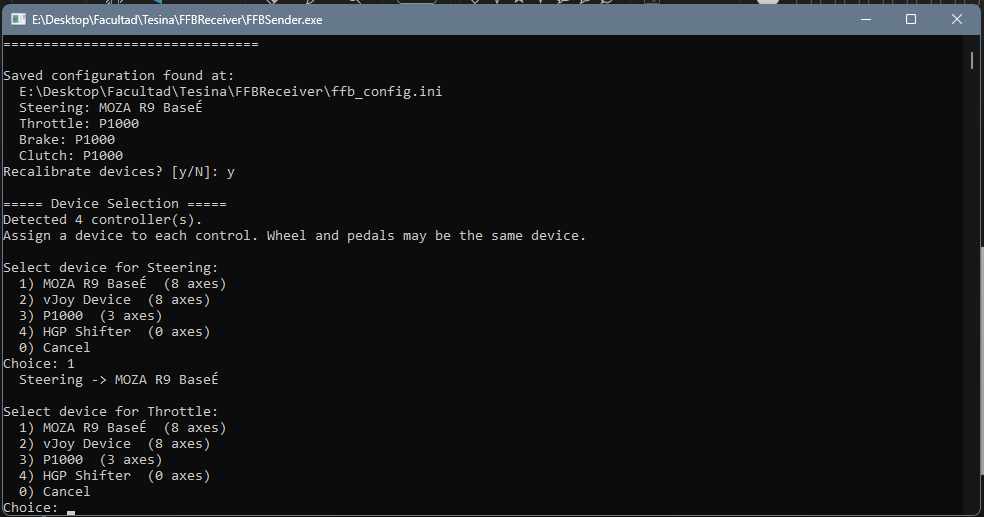
\includegraphics[width=1\textwidth]{img/device_selection.png} 
    
    \vspace{1em} % Adds spacing between image and quote
    
\caption[Selección de dispositivo]{Captura de la interfaz del sistema de envío de datos a la hora de mostrar y seleccionar el hardware para cada eje de input.}
\label{fig:device_selection}
\end{figure}


\subsection{Calibración y normalización de ejes}

Cada uno de los cuatro canales lógicos: dirección (\textit{steering}), acelerador (\textit{throttle}), freno (\textit{brake}) y embrague (\textit{clutch}), se asocia a un dispositivo y a un eje físico mediante un procedimiento de calibración interactivo de tres pasos:


\begin{enumerate}
    \item \textbf{Detección automática del eje.} Se solicita al usuario que accione el control a lo largo de todo su recorrido mientras el programa monitoriza el rango de los ocho ejes simultáneamente. El eje cuyo recorrido acumulado domina claramente sobre el resto se identifica como el eje asociado al canal. Este criterio de auto-escalado es robusto frente a diferencias de rango entre dispositivos y ante el ruido de los ejes en reposo.
    \item \textbf{Captura del rango.} Se registra el valor mínimo y máximo ($r_\text{min}$, $r_\text{max}$) alcanzado durante un barrido completo del control (de tope a tope en el volante, o de reposo a fondo en los pedales).
    \item \textbf{Confirmación de inversión.} Con una previsualización en vivo del valor normalizado, el usuario puede invertir el sentido del eje para que la convención de signo sea la correcta.
\end{enumerate}

La transformación de la lectura cruda $r$ a la señal de control normalizada aplica una función con recorte y, según el canal, una reescala bipolar o unipolar. Se define primero la fracción de recorrido:

\begin{equation}
    t = \operatorname{clamp}\!\left(\frac{r - r_\text{min}}{r_\text{max} - r_\text{min}},\; 0,\; 1\right)
\end{equation}

donde $\operatorname{clamp}(x, 0, 1)$ satura el valor al intervalo $[0, 1]$, evitando que lecturas fuera del rango calibrado produzcan salidas no deseadas. Tras aplicar opcionalmente la inversión, $t' = 1 - t$ si el eje está invertido, la salida final depende del modo del canal:

\begin{equation}
    y =
    \begin{cases}
        2\,t' - 1 & \text{modo bipolar (dirección),}\; y \in [-1, 1] \\[4pt]
        t'        & \text{modo unipolar (pedales),}\; y \in [0, 1]
    \end{cases}
\end{equation}

El modo bipolar mapea el volante de forma que su posición central corresponde a $y = 0$ y los topes a $-1$ hacia la izquierda, y $1$ hacia la derecha, el modo unipolar mapea cada pedal de forma de que la posición de reposo corresponde a $y=0$ y el fondo a $y=1$.  La configuración completa se persiste en un archivo \verb|ffb_config.ini|, de modo que la calibración solo debe realizarse una vez por configuración de hardware.\\
\newpage

\begin{figure}[htbp]
    \centering
    % Replace 'example-image' with your file name
    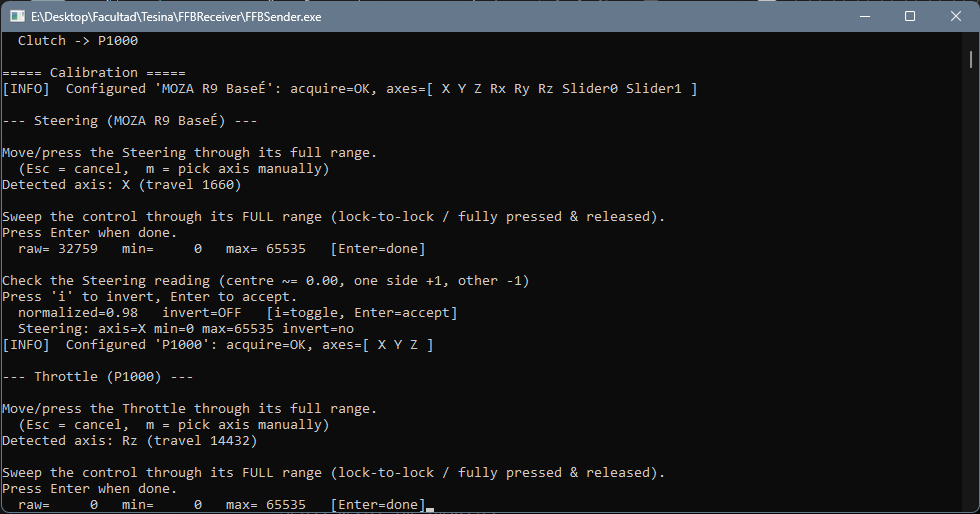
\includegraphics[width=1\textwidth]{img/calibration.png} 
    
    \vspace{1em} % Adds spacing between image and quote
    
\caption[Calibración de dispositivo]{Captura de la interfaz del sistema de envío de datos, mostrando el sistema de calibración del dispositivo.}
\label{fig:calibration}
\end{figure}


\subsection{Muestreo y transmisión en tiempo real}

El flujo de datos se obtiene ejecutando un hilo de trabajo dedicado que realiza un muestreo en intervalos determinados dependiendo de la frecuencia configurada, $\Delta t = 1000 / f_s$ ms, con un valor por defecto de $f_s = 100$ Hz que coincide con la frecuencia de sincronización en tiempo real del modelo Modelica. En cada ciclo, cada dispositivo de hardware se sondea exactamente una vez y su estado se comparte entre todos los canales (correspondientes a diferentes ejes) asociados a él. De este modo, los canales que provienen de un mismo periférico (por ejemplo, varios pedales de una misma pedalera) se muestrean de forma coherente en un único instante, sin desfase.\\

Los cuatro valores normalizados se transmiten mediante el protocolo UDP, en el caso de la computadora utilizada para las pruebas, que contiene Windows debido a la compatibilidad con los periféricos, se utiliza la biblioteca \textit{Winsock2}. Cada datagrama contiene exactamente $16$ bytes, correspondientes a cuatro números de punto flotante de $32$ bits (IEEE 754) en orden little-endian, concatenados sin cabecera:

\begin{center}
\begin{tabular}{cccc}
\hline
\textbf{Offset (bytes)} & \textbf{Longitud} & \textbf{Canal} & \textbf{Rango} \\
\hline
0  & 4 & \textit{steering} & $-1 \ldots 1$ \\
4  & 4 & \textit{throttle} & $0 \ldots 1$ \\
8  & 4 & \textit{brake}    & $0 \ldots 1$ \\
12 & 4 & \textit{clutch}   & $0 \ldots 1$ \\
\hline
\end{tabular}
\end{center}

La elección del protocolo UDP frente a TCP responde a los requisitos de una aplicación de control en tiempo real. TCP garantiza la entrega ordenada y sin pérdidas mediante confirmaciones y retransmisiones, pero a costa de una latencia variable e impredecible, un paquete perdido bloquea la entregas de los siguientes hasta su retransmisión. En un flujo de telemetría que corresponde a los inputs de un vehículo, un datagrama perdido pierde su significacncia una vez transcurrido su instante de muestreo, ya que el siguiente paquete lo reemplaza con información más reciente. UDP, al no tener confirmaciones de control ni de flujo, ofrece latencia mínima y determinista que exige la naturaleza de tener una simulación donde se tiene que poder reaccionar rápido a diferentes situaciones y que tiene que devolver feedback al conductor siendo la pérdida ocasional de un paquete un compromiso plenamente aceptable en este contexto, además de el hecho de que estos sistemas normalmente van a ejecutarse, o bien, en un mismo ordenador, o en una red local de alta velocidad, por lo que la perdida de paquetes sería mínima. \\


En el lado del receptor, el modelo Modelica lee el datagrama de $16$ bytes, desempaqueta los cuatro números de punto flotante en el mismo orden y los inyecta como las entradas \verb|steerInput|, \verb|speedInput| y \verb|brakeInput| del modelo del vehículo, cerrando así el lazo entre la acción física del conductor y la respuesta dinámica del vehículo simulado. Este canal de entrada opera de forma complementaria y en sentido inverso al flujo de salida descrito en la sección de interfaces (\verb|FrameToUDP|), que transmite la posición del vehículo hacia el visualizador.\\


Este programa fue creado como un ejemplo de una posible interfaz de entrada, como fue mencionado anteriormente, este programa puede ser reemplazado por otro, que funcione en diferentes sistemas operativos de forma nativa, o incluso en máquinas diferentes, siempre y cuando se respete el protocolo utilizado para transmitir información entre las partes del sistema.

\begin{figure}[htbp]
    \centering
    % Replace 'example-image' with your file name
    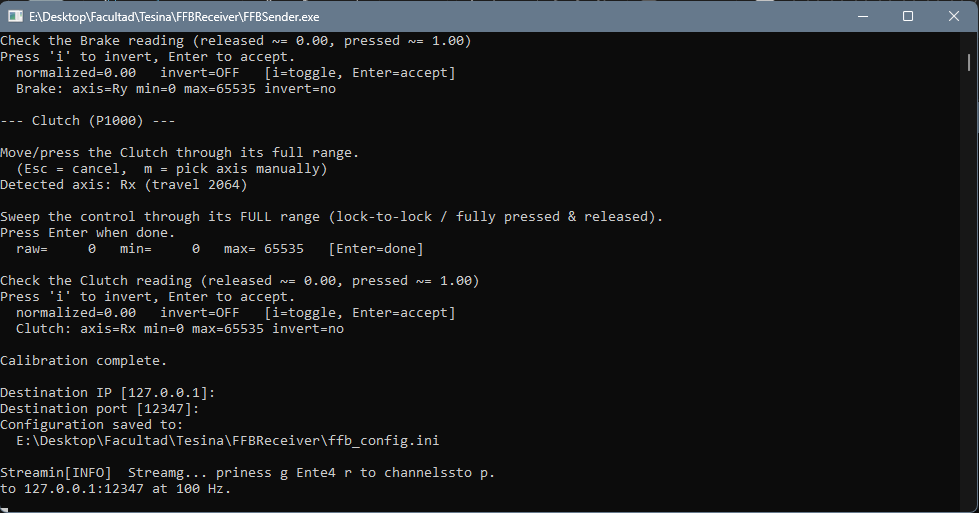
\includegraphics[width=1\textwidth]{img/running_data.png} 
    
    \vspace{1em} % Adds spacing between image and quote
    
\caption[Envío de información]{Captura de pantalla del estado del sistema de envío de datos cuando se termina la calibración de dispositivos y se comienza el envío de datos obtenidos del hardware.}
\label{fig:running_data}
\end{figure}

\section{Visualizador gráfico}
\subsection{El motor gráfico Unity}

Unity es un motor gráfco de desarrollo multiplataforma para aplicaciones interactivas en tiempo real, es ampliamente utilizado en la industria del videojuego.  Su arquitectura se organiza en torno a algunos conceptos fundamentales, definidos en su documentación oficial \cite{unity_docs}, que resultan necesarios para comprender la interfaz desarrollada:

\begin{itemize}
    \item \textbf{Escena y \textit{GameObjects}.} Una escena contiene un conjunto de objetos (\textit{GameObjects}), que son los contenedores básicos de todo elemento del mundo virtual, en este caso se utilizan para el chasis y las cuatro ruedas del auto.

    \item \textbf{Componente \textit{Transform}.} Cada \textit{GameObject} posee un componente \verb|Transform| que almacena la posición, rotación, escala y estado de jerarquía del objeto. Al modificar este componente, el objeto puede reposicionarse y reorientarse en la escena.
    
    \item \textbf{\textit{MonoBehaviour} y \textit{scripts}.} El comportamiento programable de un objeto se agrega mediante \textit{scripts} escritos en C\# que derivan de la clase base \verb|MonoBehaviour|. Esta clase expone una serie de funciones de ciclo de vida que el motor invoca automáticamente, como \verb|Start| (inicialización) y \verb|FixedUpdate| (actualización por intervalo).
    
    
    \item \textbf{Bucle de física \textit{FixedUpdate}.} A diferencia de \verb|Update|, que se ejecuta una vez por fotograma renderizado y por lo tanto su frecuencia varía dependiendo del rendimiento del computador, \verb|FixedUpdate| se invoca a intervalos fijos como parte del bucle de física del motor \cite{unity_docs} (por defecto cada 0{,}02 s, es decir, a 50 Hz), lo que garantiza un ritmo de actualización determinista, independiente de la tasa de refresco gráfico.

    
    \item \textbf{Sistema de coordenadas.} Unity emplea un sistema de coordenadas levógiro (sentido anti-horario) con el eje $Y$ apuntando hacia arriba, y representa las rotaciones internamente como cuaterniones. Esta convención difiere de la de Modelica, que es dextrógira (sentido horario) y también con $Y$ vertical, discrepancia que la interfaz debe resolver explícitamente.
\end{itemize}

\subsection{Interfaz de recepción de datos}

La interfaz que conecta Modelica con Unity se implementó como un \textit{script} de tipo \verb|MonoBehaviour| que recibe el flujo de pose emitido por el modelo de Modelica (ya sea por \verb|FrameToUDPOrientation| o por el orquestador del FMU) y lo aplica al \verb|Transform| del objeto correspondiente, modificando así su posición y orientación.  Se adjunta una instancia del \textit{script} a cada \textit{GameObject} para el chasis y cada una de las cuatro ruedas, configurando en cada una el puerto de escucha (\verb|listenPort|) para que coincida con el \verb|port_send| del transmisor Modelica asociado (12345 para el chasis y del 12346 al 12349 para las ruedas). De este modo, cada cuerpo rígido de la simulación se corresponde con un objeto de la escena y un flujo UDP dedicado.


\subsubsection*{Recepción concurrente}

La lectura de la red se ejecuta en un hilo de trabajo en segundo plano, independiente del hilo principal dedicado al renderizado del entorno. En su método \verb|Start|,  el \textit{script} abre un socket \verb|UdpClient| sobre el puerto configurado y lanza el hilo, que permanece bloqueado en la llamada de recepción a la espera de datagramas con información de posición. Esta separación es indispensable: si la recepción se realizara en el hilo principal, la llamada bloqueante detendría el renderizado hasta la llegada de cada paquete. La pose recibida se almacena en variables compartidas protegidas por un \textit{lock}, que garantiza el acceso seguro entre el hilo de red y el hilo de simulación.

\subsubsection*{Interpretación del datagrama}

Cada datagrama recibido se interpreta según el formato descrito en la sección de interfaces:  los primeros 12 bytes contienen la posición (tres flotantes de 32 bits) y, cuando el paquete alcanza los 28 bytes, los 16 bytes siguientes contienen el cuaternión de orientación (cuatro flotantes). El \textit{script} contempla ambos casos, aplicando únicamente la posición si el paquete es corto, lo que le permite operar indistintamente con los transmisores \verb|FrameToUDP| y \verb|FrameToUDPOrientation|.

\subsubsection*{Conversión de sistemas de coordenadas}

El núcleo de la interfaz es la conversión entre el sistema con sentido horario de Modelica y el de sentido anti-horario de Unity. Para la posición, la transformación consiste en negar la componente $Z$, conservando $X$ e $Y$:

\begin{equation}
    (x, y, z)_\text{Unity} = (x, y, -z)_\text{Modelica}
\end{equation}

Para la orientación, la misma inversión de eje ($S = \operatorname{diag}(1, 1, -1)$) se aplica a la rotación mediante la transformación de similitud $A_\text{Unity} = S\,A_\text{Modelica}\,S$, que sobre el cuaternión $(q_x, q_y, q_z, q_w)$, donde la parte escalar es $q_w$, equivale a negar las dos primeras componentes de la parte vectorial:

\begin{equation}
    (q_x, q_y, q_z, q_w)_\text{Modelica} \;\longrightarrow\; (-q_x, -q_y, q_z, q_w)_\text{Unity}
\end{equation}

Esta expresión fue una fuente de error durante el desarrollo: negar en su lugar la componente $q_z$ produce la rotación inversa, lo que se manifiesta visualmente como una precesión cónica del eje de giro de las ruedas en lugar de una rotación limpia.

\subsubsection*{Aplicación de la ubicación}

Finalmente, en el método \verb|FixedUpdate|, sincronizado con el bucle de física del motor, se lee la última ubicación recibida y se escribe sobre el \verb|Transform| del objeto: la posición de forma directa y la rotación componiéndola con un desfase de malla configurable (\verb|meshRotationOffset|). Este desfase corrige la discrepancia entre el eje geométrico de la malla y el eje físico del cuerpo, por ejemplo, para alinear el eje de un cilindro empleado como neumático (cuyo eje geométrico es su $Y$ local) con el eje de giro real de la rueda (su $Z$ local). El resultado es una representación tridimensional del vehículo que reproduce fielmente, y en tiempo real, la posición y la actitud calculadas por el modelo físico, incluyendo el ángulo de dirección y el giro propio de cada rueda.

\begin{figure}[htbp]
    \centering
    % Replace 'example-image' with your file name
    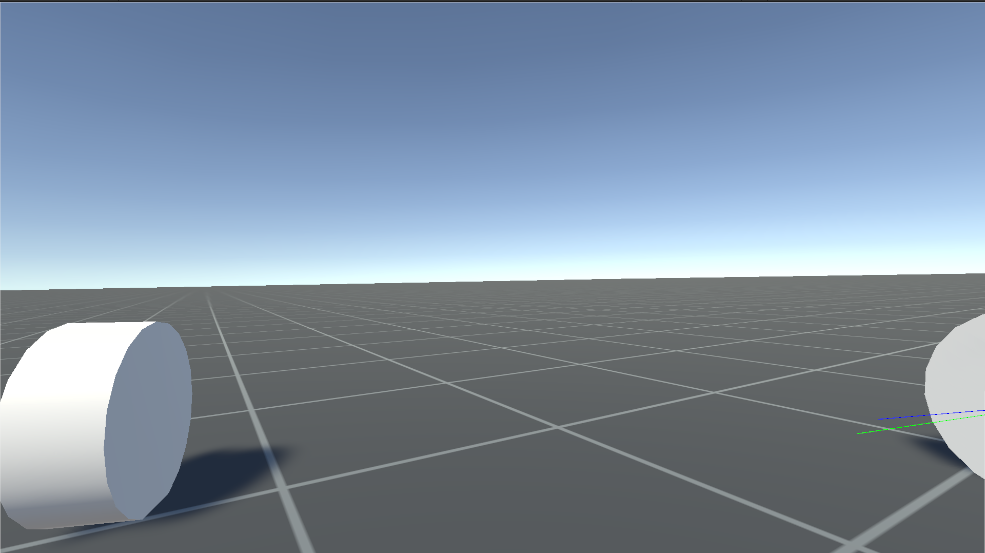
\includegraphics[width=1\textwidth]{img/unity.png} 
    
    \vspace{1em} % Adds spacing between image and quote
    
\caption[Entorno de Unity]{Captura de pantalla de la interfaz sencilla de Unity sincronizada con la información obtenida del modelo de Modelica. Se puede observar un entorno plano, con la cámara aproximadamente en la posición del conductor, y las dos ruedas delanteras moviéndose acorde a la dinámica del vehículo.}
\label{fig:running_data}
\end{figure}
\newpage


\section{Arquitectura de co-simulación}
\label{sec:cosim}

Las tres componentes explicadas hasta ahora deben ejecutarse simuláneamente e intercambiar información al ritmo configurado para el lazo/simulación. La forma aparentemente más directa, y que se tomó como primer acercamiento, fue usar las herramientas presentadas para que envíen y reciban paquetes UDP mediante los bloques del paquete \verb|Interfaces|. Esta sección explica por qué esa vía resultó inviable con el compilador empleado y describe la arquitectura que finalmente se adoptó.

\subsection{Por qué el modelo no puede cerrar el lazo por sí mismo}

Un lazo cerrado que incluye interacción humana necesita muestrear su entrada, el comando del conductor llega en instantes discretos y debe mantenerse constante entre ellos. En Modelica, esto se representa con una cláusula \verb|when sample(...)|, presente tanto en \verb|UDPReceive| como en \verb|UDPSend| y en \verb|RealtimeSynchronize|.

El hallazgo que determinó el cambio en la arquitectura original fue que la simple presencia de un reloj periódico de muestreo en el modelo impide a CVODE integrar más allá de un lapso de tiempo determinado, en este caso fueron diecinueve segundos. Cabe remarcar que algunos cambios en la interfaz de entrada/salida hacían que ese valor cambie, pero con un mismo modelo, este siempre abortaba al mismo instante de tiempo. Esto no se debe a un problema del modelo del vehículo ni del volumen de datos, este mismo error se puede replicar colocando tres bloques \verb|Sampler| transmitiendo valores constantes, sin conexión alguna con el resto del sistema.  El Apéndice~\ref{sec:appendix} documenta el caso mínimo de reproducción.

 % El Apéndice~\ref{sec:appendix} documenta el caso mínimo de reproducción junto con los otros dos defectos del compilador que se encontraron en el curso de este trabajo.

Dado que muestrear dentro del modelo es la causa del problema, la solución consistió en moverlo fuera del sistema de ecuaciones.


% \subsection{Un paso intermedio: comunicación sin Modelica\_DeviceDrivers}

% Antes de llegar a esa conclusión se implementaron versiones de los bloques de comunicación que reemplazan la cadena de \textit{Modelica\_DeviceDrivers} por una única función externa en C. El modelo \verb|UDPInputDirect| sustituye la secuencia \verb|UDPReceive| seguida de cuatro \verb|GetFloat| por una función \verb|udpRead4| que abre un \textit{socket} no bloqueante, lo drena y devuelve el último datagrama disponible; \verb|FrameToUDPDirect| hace lo propio en el sentido de la transmisión con una función \verb|udpSend7|. Ambas conservan el formato de los paquetes, de modo que los programas del otro extremo no requieren modificación alguna.

% Estas versiones eliminan una falla distinta y anterior —una detención a los $2{,}6$ s con los bloques originales— y reducen el sistema en unas $620$ ecuaciones, pero no resuelven la limitación de fondo: siguen necesitando un reloj de muestreo. Se conservan en la biblioteca porque suprimen la dependencia de una biblioteca externa en el camino crítico y porque documentan el defecto en ambos sentidos de la comunicación.

\subsection{El modelo como FMU de intercambio de modelos}

La solución implementada consiste en exportar el modelo del vehículo como una \textit{Functional Mock-up Unit} (FMU) siguiendo el estándar FMI~2.0, y trasladar el muestreo, la integración y la sincronización a una aplicación externa. El modelo se convierte en una biblioteca que contiene una función de avance explícita, es decir, nada sucede en él hasta que el programa que lo instancia se lo pida.

Se emplea la variante de intercambio de modelos (\textit{Model Exchange}) y no la de co-simulación. Un FMU de co-simulación incluye a su propio integrador, lo que resulta más cómodo, pero los generados por  OpenModelica~1.25.5 terminan abruptamente durante el avance de la integración. Por lo que para agilizar el desarrollo, se utilizó este tipo de FMU que no contiene integrador, si no que expone las derivadas del estado y es la aplicación externa la que integra, lo que permite utilizar una implementación independiente que no presenta problemas.

El modelo exportado (\verb|Examples.CarExport|) es un wrapper del vehículo y del entorno en el que se encuentra, y expone hacia afuera tres entradas \verb|steer|, \verb|throttle| y \verb|brake|, además de que por cada uno de los cinco cuerpos (cuatro ruedas y el chasis) expone su posición en el sistema de referencia global, con su orientación. Esto resulta en un modelo que expone lo mismo que se recibía/enviaba por UDP pero sin contener bloques de comunicación, ni de muestreo y con la animación deshabilitada para obtener un mejor desempeño.

La orientación se exporta como una matriz de rotación de nueve componentes y no como cuaternión. El motivo es por una falla del compilador: la conversión \verb|Frames.to_Q| hace fallar al generador de código FMI con un error de dimensiones incompatibles aunque el mismo modelo compila y simula sin dificultad como ejecutable autónomo. La conversión a cuaternión para compatibilizarlo con el visualizador se hace en la aplicación de control, copiando la implementación de \verb|Quaternions.from_T| para que el paquete transmitido resulte idéntico al que emitía el modelo original.


% La exportación se automatiza con un guion que fija la configuración necesaria:

% \begin{verbatim}
% buildModelFMU(DDynamics.Examples.CarExport.CarExport,
%               version = "2.0", fmuType = "me",
%               fileNamePrefix = "CarExport", platforms = {"static"});
% \end{verbatim}

% Conviene señalar dos detalles que no son evidentes. La instrucción es \verb|buildModelFMU| y no \verb|translateModelFMU|: esta última solo traduce el modelo, informa éxito y no genera archivo alguno. Y la opción \verb|platforms| con el valor \verb|static| enlaza el binario de forma estática, de modo que el FMU no dependa de que las bibliotecas dinámicas de OpenModelica estén disponibles al momento de ejecutarlo.

\subsection{La aplicación de control}

La aplicación de control (o \textit{master}) es el programa que se encarga de controlar el lazo. Se ubica entre la interfaz de hardware y el visualizador, comunicándose con ambos por UDP, según muestra la Figura~\ref{fig:cosim}.

\begin{figure}[H]
\centering
\begin{tikzpicture}[font=\small,
    box/.style={draw, rounded corners=2pt, minimum height=1.2cm,
                align=center, inner sep=6pt},
    ar/.style={-{Latex[length=2mm]}, thick}]

  \node[box, fill=black!5]  (ffb) at (0,0)   {\texttt{FFBSender}\\{\footnotesize volante y pedales}};
  \node[box, fill=black!12, line width=1pt] (mas) at (6,0) {aplicación de control\\{\footnotesize FMU + integrador}};
  \node[box, fill=black!5]  (uni) at (12,0)  {Unity\\{\footnotesize visualizador}};

  \draw[ar] (ffb) -- node[above, font=\scriptsize, align=center]
      {UDP 12344\\$4\times$float32} (mas);
  \draw[ar] (mas) -- node[above, font=\scriptsize, align=center]
      {UDP 12345--12349\\$7\times$float32} (uni);
\end{tikzpicture}
\caption[Arquitectura de co-simulación]{Arquitectura del lazo cerrado. El muestreo, la integración y la sincronización con el reloj de pared ocurren en la aplicación de control, fuera del sistema de ecuaciones del modelo. Los formatos de los paquetes son los que ya emitía y esperaba cada extremo, de forma que ni la interfaz de hardware ni el visualizador requirieron modificación.}
\label{fig:cosim}
\end{figure}

Su bucle principal, con un paso de comunicación configurable de $10$ ms por defecto, realiza en cada iteración cuatro operaciones: escribe en el FMU el último comando recibido, avanza la integración en un paso, lee las poses de los cinco cuerpos, las encola para su transmisión y espera hasta el instante que indique su frecuencia. 

 % El comando se mantiene constante durante todo el paso, lo que constituye el mismo retenedor de orden cero que antes rompía a CVODE, con la diferencia esencial de que ahora ocurre entre llamadas al integrador y no como un evento temporal dentro de las ecuaciones.

La aplicación se estructura en tres hilos: uno para recibir los comandos del conductor, otro para ejecutar la integración y el último que se encarga de transmitir las poses. La principal ventaja de esto es que una lectura bloqueante de red no detiene la ejecución del integrador.



% Dos decisiones de diseño merecen mención. El hilo de recepción conserva únicamente el datagrama más reciente y descarta los anteriores: en un lazo en tiempo real un comando viejo no tiene valor alguno. Y un vigilante anula los comandos si no llega ningún datagrama durante medio segundo, de modo que la caída del programa de adquisición no deje aplicado indefinidamente el último valor de acelerador.


\subsection{Bibliotecas empleadas en la aplicación de control}

La aplicación de control se implementó en Python. La estructura de comunicación y concurrencia se resuelve utilizando la biblioteca estándar del lenguaje, sin incluir dependencias externas. La única dependencia de tercero es la que permite el acceso al modelo.

\subsubsection{FMPy}

FMPy es una implementación del estándar FMI en Python \cite{fmpy} y es la que permite cargar el FMU e interactuar con él. Se emplean dos componentes: el primero es la interfaz de bajo nivel \verb|FMU2Model|, que expone directamente las funciones de la norma (fijar entradas, leer y escribir el vector de estados, obtener las derivadas y los indicadores de evento, gestionar el modo de eventos). Se recurre a esta interfaz y no a la de simulación por lotes porque el lazo cerrado requiere inyectar comandos entre pasos sucesivos, algo que una llamada por lotes no permite.

El segundo componente utilizado es \verb|CVodeSolver|, un enlace a la biblioteca SUNDIALS \cite{hindmarsh2005} que provee el integrador CVODE \cite{cohen1995}. Este es el mismo algoritmo empleado en OpenModelica, pero con una implementación y entorno diferente, lo que nos permite evitar ciertos problemas que presentaba el entorno de OpenModelica, que resultaron claves para la ejecución de algunos experimentos.

 % es precisamente esa independencia la que permite eludir los defectos del entorno de OpenModelica documentados en el Apéndice~\ref{sec:appendix}.


% \subsubsection{El estándar FMI}

% El formato de intercambio está definido por la especificación 

% \paragraph{El estándar FMI.} El formato de intercambio está definido por la especificación FMI~2.0 \cite{blochwitz2012}, que fija tanto la estructura del archivo —el descriptor \verb|modelDescription.xml| y los binarios compilados— como la interfaz en C que el FMU expone. Que ambos extremos se atengan a un estándar es lo que hace posible combinar un modelo generado por OpenModelica con un integrador provisto por otra herramienta.

\subsubsection{Sobre la elección del lenguaje}
Utilizar el lenguaje Python para controlar el lazo en tiempo real merece justificación. Las únicas operaciones que la aplicación ejecuta en Python puro son la lectura de las poses, su conversión a cuaternión y una llamada a un callback de la librería SUNDIALS, que consumen entre el $5$ y el $7\%$ del tiempo de cada iteración. El resto del costo corresponde a la integración, que ocurre dentro del código compilado en C de SUNDIALS. La elección del lenguaje entonces no penaliza demasiado el desempeño y además simplifica la instrumentación y los experimentos. Cabe además aclarar, que si se requiere obtener más desempeño en el sistema, esta aplicación puede ser reemplazada por otra compilada en algún otro lenguaje, siempre y cuando respete los estándares de comunicación entre las partes y el protocolo FMI~2.0 \cite{blochwitz2012}.

% Emplear un lenguaje interpretado para gobernar un lazo en tiempo real merece justificación, y la medición la aporta. Las únicas operaciones que la aplicación ejecuta en Python puro son la lectura de las poses, su conversión a cuaternión y una llamada a un callback de la librería SUNDIALS, que consumen entre el $5$ y el $7\,\%$ del tiempo de cada iteración. La totalidad del costo restante corresponde a la integración, que ocurre dentro del código compilado en C FMU. La elección del lenguaje no penaliza, por lo tanto, el desempeño del lazo, y a cambio simplifica notablemente la instrumentación y los experimentos.


\subsection{Consecuencias de la arquitectura}

El resultado es un sistema en el que el modelo deja de incluir bloques de comunicación y sincronización y en el que las tres partes del sistema se comunican exclusivamente mediante UDP con formatos fijos. Se mantiene la libertad de poder modificar cualquiera de ellas sin tocar al resto: el programa de adquisición podría reemplazarse por otro periférico o por una entrada sintética, y el visualizador por un motor gráfico distinto, siempre que respeten los formatos de la Figura~\ref{fig:cosim}. 

Realizar este cambio, sumado a pasar la responsabilidad de la sincronización con el tiempo real a la aplicación de control, simplifica la arquitectura del modelo en Modelica, dejando solamente que este se encargue de cumplir su función principal: modelar un sistema físico, y dejando las funcionalidades de red a otros programas que estén más adaptados a cumplir esas responsabilidades.

% La sincronización con el tiempo real pasa a ser una espera en el bucle de la aplicación de control, por lo que el bloque \verb|RealtimeSynchronize| pasa a ser innecesario, lo que elimina el pro

% El acompasamiento con el tiempo real pasa a ser una espera en el bucle de la aplicación de control, lo que además vuelve innecesario el bloque \verb|RealtimeSynchronize| y elimina el problema de tener cinco instancias del mismo compitiendo por acompasar una única simulación. La contrapartida es que la responsabilidad de la integración —la elección del integrador, su tolerancia y el tamaño del paso de comunicación— se traslada del compilador a la aplicación, y con ella la necesidad de caracterizar su desempeño, que es el objeto del Capítulo~\ref{sec:experiments}.
